\documentclass[a4paper,10pt]{IEEEtran}
\newcommand{\DocTitleText}{Chase Combining Hybrid \myARQ{} Type \myII{} Cross-Layer Optimization for Underlay Cognitive Radio}
\newcommand{\DocAuthorBlock}{\IEEEauthorblockA{Vaddadi V.~K.~Praneeth, Nour Mansour and Dirk Dahlhaus}}
\newcommand{\DocAffiliation}{\IEEEauthorblockN{Communications Laboratory, University of Kassel}}
\newcommand{\DocEmails}{ Web: www.uni-kassel.de; Email:\{praneeth,mansour,dahlhaus\}@uni-kassel.de}


\usepackage{silence}
\WarningFilter{latex}{Command \showhyphens has changed}
\WarningFilter{caption}{Unknown document class}
\usepackage{cite}
\usepackage{amsmath,amssymb,amsfonts}
\usepackage{graphicx}
\usepackage{textcomp}
\usepackage{balance}
\usepackage{float}  
\usepackage[hidelinks]{hyperref}
\let\labelindent\relax
\usepackage{mathtools,bm}
\usepackage{array,multirow,booktabs}
\usepackage{lipsum}
\usepackage{hyphenat}
\usepackage{caption}
\usepackage{microtype}
\usepackage{psfrag}
\usepackage{enumitem}
\usepackage[utf8]{inputenc}
\usepackage{xcolor}

\newcommand{\mySU}{SU} % Secondary User
\newcommand{\myPU}{PU} % Primary User
\newcommand{\myUCRS}{UCRS} % Underlay Cognitive Radio System
\newcommand{\myUS}{US} % User Scheduling
\newcommand{\myPHY}{PHY} % Physical Layer
\newcommand{\myDLC}{DLC} % Data Link Control Layer
\newcommand{\myCLO}{CLO} % Cross-Layer Optimization
\newcommand{\mySE}{SE} % Spectral Efficiency
\newcommand{\myQoS}{QoS} % Quality of Service
\newcommand{\myBEP}{BEP} % Bit Error Probability
\newcommand{\myPEP}{PEP} % Packet Error Probability
\newcommand{\mySINR}{SINR} % Signal-to-Interference-plus-Noise Ratio
\newcommand{\myTHARQ}{THARQ} % Truncated Hybrid ARQ
\newcommand{\myCC}{CC} % Chase Combining
\newcommand{\myARQ}{ARQ} % Automatic Repeat reQuest
\newcommand{\myCRC}{CRC} % Cyclic Redundancy Check
\newcommand{\myCA}{CA} % Coding Adaptation
\newcommand{\myJBPL}{JBPL} % Joint Bit and Power Loading
\newcommand{\myLDPC}{LDPC} % Low-Density Parity Check
\newcommand{\myABICM}{ABICM} % Adaptive Bit-Interleaved Coded Modulation
\newcommand{\myABICMinv}{\ensuremath{\mathrm{ABICM}^{-1}}} % Inverse ABICM
\newcommand{\myQAM}{QAM} % Quadrature Amplitude Modulation
\newcommand{\myTF}{TF} % Time-Frequency
\newcommand{\mySFB}{SFB} % Subcarrier Feedback
\newcommand{\myAFB}{AFB} % Adaptive Feedback
\newcommand{\myEGC}{EGC} % Equal Gain Combining
\newcommand{\myChannelEstimator}{channel estimator} % Channel Estimator
\newcommand{\myI}{I} % Indicator
\newcommand{\myII}{II} % Type II
\newcommand{\myRV}{RV} % Random Variable
\newcommand{\myPDF}{PDF} % Probability Density Function
\newcommand{\myGA}{GA} % Genetic Algorithm
\newcommand{\myMATLAB}{MATLAB} % MATLAB Software

\newcommand{\mymax}{\mathrm{max}} % Maximum
\newcommand{\myK}{K} % Number of Subcarriers
\newcommand{\myX}{X} % Random Variable X
\newcommand{\myA}{A} % Random Variable A
\newcommand{\myJ}{J} % Transmission Index
\newcommand{\myi}{i} % Index i
\newcommand{\myH}{H} % Channel Coefficient
\newcommand{\mybrm}{\mathrm{b}} % Bit
\newcommand{\myP}{P} % Power
\newcommand{\myUBrm}{\mathrm{UB}} % Upper Bound
\newcommand{\myw}{w} % Weight
\newcommand{\myf}{f} % Function f

\newcommand{\myun}{un} % Uncoded
\newcommand{\myco}{co} % Coded
\newcommand{\myunrm}{\mathrm{un}} % Uncoded (roman)
\newcommand{\mycorm}{\mathrm{co}} % Coded (roman)

\newcommand{\myG}{G} % Gaussian RV sum
\newcommand{\mypac}{pac} % Packet
\newcommand{\mypacrm}{\mathrm{\mypac}} % Packet (roman)
\newcommand{\myreq}{req} % Requirement
\newcommand{\myreqrm}{\mathrm{\myreq}} % Requirement (roman)
\newcommand{\mydB}{dB} % Decibel
\newcommand{\myIII}{III} % Type III
\newcommand{\mydBrm}{\mathrm{dB}} % dB (roman)
\newcommand{\myMreq}{\myM_{\myreqrm}} % Minimum required bits
\newcommand{\YSellzeroj}{\ensuremath{\myY_{\myS,\ell,0,\myj}}} 
\newcommand{\YSellonej}{\ensuremath{\myY_{\myS,\ell,1,\myj}}}
\newcommand{\YSellKj}{\ensuremath{\myY_{\myS,\ell,\myK-1,\myj}}}
\newcommand{\YSjelk}{\ensuremath{\myY^{(\myj)}_{\myS,\ell,\myk}}}

\newcommand{\myQAMdemod}{\begin{tabular}{c}\myQAM{}\\demodulator\end{tabular}}
\newcommand{\myDeinterleaver}{deinterleaver}
\newcommand{\myLDPCdecoder}{\begin{tabular}{c}\myLDPC{}\\decoder\end{tabular}}

\newcommand{\myCRCcheck}{\begin{tabular}{c}\myCRC\\check\end{tabular}}
\newcommand{\myPass}{pass} % CRC pass
\newcommand{\myFail}{fail} % CRC fail

\newcommand{\myB}{B} % Bit
\newcommand{\myBhatkhat}{\ensuremath{\hat{\myB}_{\kappa}}} % Estimated bit
\newcommand{\myRC}{R_c} % Code rate
\newcommand{\mytotrm}{\mathrm{tot}} % Total
\newcommand{\myMtot}{\myM_{\mytotrm}} % Total constellation points
\newcommand{\myBlk}{\myB_{\ell,\myk}} % Block bit

\newcommand{\myJDots}{%
  \scriptsize
  \begin{tabular}{@{}c@{}}
    $\cdot$\\[-1.5ex]
    $\cdot$\\[-1.5ex]
    $\cdot$
  \end{tabular}%
} % Vertical ellipsis
\newcommand{\myy}{y} % generic y variable
\newcommand{\myD}{D} % generic D variable
\newcommand{\myb}{b} % generic b variable
\newcommand{\mya}{a} % generic a variable
\newcommand{\myL}{L} % number of packets/blocks
\newcommand{\myd}{d} % distance / Hamming weight
\newcommand{\myu}{u} % unit step function

\newcommand{\myAbf}{\mathbf{A}} % matrix A
\newcommand{\mypbf}{\mathbf{p}} % power vector
\newcommand{\mymbf}{\mathbf{m}} % modulation pattern vector
\newcommand{\myminmathrm}{\mathrm{min}} 
\newcommand{\myQAMrm}{\mathrm{\myQAM}} 
\newcommand{\mytemprm}{\mathrm{temp}} 
\newcommand{\mytriprm}{\mathrm{trip}} 
\newcommand{\myp}{p} % generic power
\newcommand{\myS}{S} 
\newcommand{\mySrm}{\mathrm{S}} 
\newcommand{\SSellZeroj}{\ensuremath{\myS_{\mySrm,\ell,0,\myj}}} 
\newcommand{\SSellOnej}{\ensuremath{\myS_{\mySrm,\ell,1,\myj}}} 
\newcommand{\SSellKj}{\ensuremath{\myS_{\mySrm,\ell,\myK-1,\myj}}} 
\newcommand{\SSelk}{\myS_{\mySrm,\ell,\myk}} 

\newcommand{\Dlk}{\myD_{\ell,\myk}} 
\newcommand{\myHcal}{\mathcal{H}} % channel coefficients
\newcommand{\myParGen}{parameter generator}

\newcommand{\myR}{R} % rate
\newcommand{\myRhat}{\hat{\myR}} % estimated rate

\newcommand{\myc}{c} % generic constant
\newcommand{\myz}{z} % generic complex variable

\newcommand{\myoptrm}{\mathrm{opt}} % optimal
% Channel matrices
\newcommand{\HPP}{\ensuremath{\myHcal_{\myPrm\myPrm}}} % PU-PU channel
\newcommand{\HPS}{\ensuremath{\myHcal_{\myPrm\mySrm}}} % PU-SU channel
\newcommand{\HSP}{\ensuremath{\myHcal_{\mySrm\myPrm}}} % SU-PU channel
\newcommand{\HSS}{\ensuremath{\myHcal_{\mySrm\mySrm}}} % SU-SU channel
\newcommand{\IPjn}{\ensuremath{\myImath_{\myPrm,\myj}[\myn]}} % PU interference
\newcommand{\WPjn}{\ensuremath{\myW_{\myPrm,\myj}[\myn]}} % PU noise
\newcommand{\ISjn}{\ensuremath{\myImath_{\mySrm,\myj}[\myn]}} % SU interference
\newcommand{\WSjn}{\ensuremath{\myW_{\mySrm,\myj}[\myn]}} % SU noise

\newcommand{\myRX}{RX} % receiver
\newcommand{\myTX}{TX} % transmitter
\newcommand{\myBL}{BL} % bit loading
\newcommand{\myDFTFB}{DFT-FB} % DFT filter bank
\newcommand{\myTPI}{TPI} % total power interference
\newcommand{\mySCP}{SCP} % symbol cyclic prefix
\newcommand{\myPL}{PL} % path loss

\newcommand{\myHtilde}{\tilde{H}} % normalized channel coefficient

\newcommand{\myLBrm}{\mathrm{LB}} % lower bound

% Expected value notation
\newcommand{\myE}[2][]{\mathbf{E}_{#1}\!\left\{#2\right\}} % expectation
\newcommand{\EX}[2]{\mathrm{E}_{#1}\!\left\{#2\right\}} % alternative notation

% Inner product / conditional / set notation
\newcommand{\inner}[2]{\left\langle #1, #2 \right\rangle} % inner product
\newcommand{\cond}[3]{#1 \!\mid\! (#2 = #3)} % conditional
\newcommand{\set}[1]{\left\{#1\right\}} % set
\newcommand{\myM}{M} % modulation order
\newcommand{\myNbb}{\mathbb{N}} % natural numbers
\newcommand{\myZbb}{\mathbb{Z}} % integers
\newcommand{\myRbb}{\mathbb{R}} % real numbers

\newcommand{\myx}{x} % generic x

\newcommand{\myOmegaZeroK}{\Omega_{0,K}} % Frequency bin set from 0 to K-1

\newcommand{\mySSellk}{\myS_{\mySrm,\myell,\myk}} % SU transmitted symbol at time slot ℓ and subcarrier k
\newcommand{\mygellk}[1]{\myg_{\myell,\myk}[#1]} % Pulse shaping filter g at slot ℓ, subcarrier k, sample #
\newcommand{\mySSn}{\myS_{\mySrm}[\myn]} % SU transmitted symbol at discrete time n

\newcommand{\J}{J} % Transmission index
\newcommand{\Jmax}{\myJ_{\mathrm{max}}} % Maximum number of transmissions

\newcommand{\YSelkj}{\myY_{\mySrm,\ell,\myk,\myj}} % Received SU signal at slot ℓ, subcarrier k, transmission j

\newcommand{\myFB}{FB} % Feedback

\newcommand{\YSelkjp}{\myY_{\mySrm,\ell,\myk,{\myj}'}} % Received SU signal at slot ℓ, subcarrier k, previous transmission j'
\newcommand{\HSSelkj}{\myH_{\mySrm\mySrm,\ell,\myk,\myj}} % SU-to-SU channel at slot ℓ, subcarrier k, transmission j
\newcommand{\XPSelkj}{\myX_{\myPrm\mySrm,\ell,\myk,\myj}} % PU-to-SU transmitted signal at slot ℓ, subcarrier k, transmission j
\newcommand{\ISelkj}{\myImath_{\mySrm,\ell,\myk,\myj}} % Interference at SU for slot ℓ, subcarrier k, transmission j
\newcommand{\WSelkj}{\myW_{\mySrm,\ell,\myk,\myj}} % Noise at SU for slot ℓ, subcarrier k, transmission j

% Indexing set notation
\newcommand{\Omegaset}[2]{%
  \Omega_{#1,#2} = \set{n \in \myZbb : #1 \le n \le #1 + #2 - 1} % Set of indices from #1 to #1+#2-1
}

\newcommand{\HSSelkjp}{\myH_{\mathrm{SS},\ell,\myk,{\myj}'}} % SU-to-SU channel for previous transmission j'
\newcommand{\HSSelkjpconj}{\myH^{*}_{\mySrm\mySrm,\ell,\myk,{\myj}'}} % Conjugate of SU-to-SU channel for previous transmission j'

\newcommand{\ASSkj}{\myA^{(\myj)}_{\mySrm,\myk}} % SU SINR after j transmissions on subcarrier k

\newcommand{\HSSkjt}{\widetilde{H}_{\mySrm\mySrm,\myk,{\myj}'}} % Time-invariant SU channel estimate
\newcommand{\HPSkjt}{\widetilde{H}_{\myPrm\mySrm,\myk,{\myj}'}} % Time-invariant PU-to-SU channel estimate

\newcommand{\figscale}{0.6} % Scaling factor for figures
\newcommand{\figtext}[1]{\scalebox{\figscale}{#1}} % Scale figure text

\newcommand{\myg}{g} % Pulse shaping filter

\newcommand{\myQAMmodulator}{\scalebox{0.6}{\shortstack{\myQAM{}\\modulator}}} % QAM modulator block
\newcommand{\myInterleaver}{\scalebox{0.6}{interleaver}} % Interleaver block
\newcommand{\myLDPCencoder}{\scalebox{0.6}{\shortstack{\myLDPC{}\\encoder}}} % LDPC encoder block

\newcommand{\myell}{\ell} % Time slot index
\newcommand{\myj}{j} % Transmission index
\newcommand{\myk}{k} % Subcarrier index
\newcommand{\abs}[1]{\lvert #1\rvert} % Absolute value

\newcommand{\pP}{\myp_{\myPrm}} % PU transmit power
\newcommand{\myPrm}{\mathrm{P}} % Primary user notation

\newcommand{\myCcal}{\mathcal{C}} % Codebook set
\newcommand{\myNcal}{\mathcal{N}} % Noise set
\newcommand{\myF}{F}  % Generic function F
\newcommand{\myWSS}[0]{WSS} % Wide Sense Stationary
\newcommand{\mypow}[1]{p_{#1}} % Power allocation

\newcommand{\mySS}[3]{S_{S,#1,#2,#3}} % SU transmitted symbol at indices

\newcommand{\gkl}{\myg_{\ell,\myk}[\myn]} % Pulse g at slot ℓ, subcarrier k, time n
\newcommand{\gshift}{g[n-K\ell]\,e^{\,i\frac{2\pi}{K} nk}} % Time-shifted pulse for OFDM
% Sequence notations
\newcommand{\myn}{n} % sequence length
\newcommand{\SPn}{\ensuremath{\myS_{\myPrm}[\myn]}} % PU sequence
\newcommand{\SSn}{\ensuremath{\myS_{\mySrm}[\myn]}} % SU sequence

\newcommand{\myTrm}{\mathrm{T}} % transpose
\newcommand{\mym}{m} % modulation order
\newcommand{\myY}{Y} % received signal

% Received signals
\newcommand{\YPjn}{\ensuremath{\myY_{\myPrm,\myj}[\myn]}} % PU received signal
\newcommand{\YSjn}{\ensuremath{\myY_{\mySrm,\myj}[\myn]}} % SU received signal

\newcommand{\myImath}{I} % interference
\newcommand{\myW}{W} % noise
\newcommand{\OmegaRc}{\Omega_{R_c}}
% ===== Parameters for Performance Analysis =====

\newcommand{\rbRc}{R_c}                 % code rate
\newcommand{\rbsigmaSW}{\sigma_{\mathrm{S},\mathrm{W}}}
\newcommand{\rbK}{K}                    % number of subcarriers
\newcommand{\rbOmega}{\Omega_{0,K}}     % index set
\newcommand{\rbpk}{p_k}                 % power on subcarrier k
\newcommand{\rbsigmaSSk}{\sigma_{SS,k}} % SU-SU channel variance
\newcommand{\rbmk}{m_k}                 % modulation order per subcarrier
% ===== System Parameters =====
\newcommand{\rbMtot}{M_{\mathrm{tot}}}

% ===== Spectral Efficiency Bounds =====
\newcommand{\rbSLB}{S_{\mathrm{LB}}}

% ===== Coding Rate =====
% --- Example definitions for LaTeX commands ---
\newcommand{\BGTwo}{Base Graph 2}       % اسم مصفوفة التحقق
\newcommand{\LiftSize}{384}             % حجم الرفع
\newcommand{\BaseRate}{1/3}             % معدل الكود الأساسي
\newcommand{\RateSet}{\{1/3, 1/2, 2/3, 3/4\}}  % مجموعة معدلات الكود
\newcommand{\GA}{genetic algorithm}     % اختصار GA
\newcommand{\Mreq}{M_{\text{req}}}      % الحد المطلوب للـ QoS
\newcommand{\JmaxVal}{2}                % الحد الأقصى لعدد الإعادة
\newcommand{\preqVal}{0.1}              % احتمال الخطأ المطلوب
% --- Transmit powers ---
\newcommand{\ptot}{p_{\mathrm{tot}}}       % Total SU TX power
\newcommand{\pp}{p_{\mathrm{P}}}           % PU TX power

% --- Subcarriers and symbols ---
\newcommand{\Mtot}{M_{\mathrm{tot}}}       % Total number of symbols
\newcommand{\K}{K}                          % Number of subcarriers
\newcommand{\Lsym}{L}                       % Number of multicarrier symbols

% --- Noise and interference ---
\newcommand{\sigmaPW}{\sigma_{\mathrm{P},\mathrm{W}}^2} % PU thermal noise
\newcommand{\sigmaSW}{\sigma_{\mathrm{S},\mathrm{W}}^2} % SU thermal noise
\newcommand{\sigmaSP}{\sigma_{\mathrm{SP}}^2}           % SU→PU interference
\newcommand{\sigmaPS}{\sigma_{\mathrm{PS}}^2}           % PU→SU interference
\newcommand{\sigmaPIk}{\sigma_{\mathrm{P},I,k}^2}      % PU TPI profile
\newcommand{\sigmaSIk}{\sigma_{\mathrm{S},I,k}^2}      % SU TPI profile

% --- Interference temperature ---
\newcommand{\iTemp}{i_{\mathrm{temp}}}     % Interference temperature
\newcommand{\betaVal}{\beta}               % Interference margin
\newcommand{\preq}{p_{\mathrm{req}}}       % Required probability for QoS
\newcommand{\rbRcopt}{\hat{R}_{\mathrm{c,opt}}}  % Optimum coding rate
% --- Preamble or before \begin{document} ---
\newcommand{\rbJmax}{J_\text{max}}              % Max transmissions
\newcommand{\rbMreq}{M_\text{req}}              % Required symbols
\newcommand{\rbpreq}{p_\text{req}}              % Required probability
\newcommand{\rbEtaDB}{\eta}                     % Average energy per bit (dB)






\microtypesetup{stretch=20,shrink=20}
\color{black!80}
\makeatletter
\def\tablename{Table}
\makeatother
\setlength{\columnsep}{16pt}    

\begin{document}

\title{\DocTitleText}
\author{\DocAuthorBlock\\\DocAffiliation\\\DocEmails}

\maketitle
\pagestyle{empty}
\thispagestyle{empty}

\setlength{\parindent}{0em}
\begin{abstract}
A novel cross-layer optimization (\myCLO{}) scheme to
significantly enhance the spectral efficiency (\mySE{}) of a secondary
user (\mySU{}) transmission in an underlay cognitive radio system
(\myUCRS{}) is proposed. The scheme jointly optimizes the physical
layer (\myPHY{}) and data link control layer (\myDLC{}) of the \mySU{}~trans-\linebreak
mission. At the \myPHY{}, a joint \!bit and power loading \!(\myJBPL{})~with
coding adaptation (\myCA{}) using rate-matched low-density-parity-
check (\myLDPC) coding is employed. A truncated hybrid automatic
repeat request (\myTHARQ{}) using chase combining (\myCC{}), known~as
\myARQ{} type \myII{}, is implemented at the \myDLC{}.An analytic lower~bound\linebreak
on \!the \!\mySE{} for coded transmission is derived and maximized subject
to different quality-of-service (\myQoS{}) and stochastic chance-based
constraints as well as third-party colored Gaussian interference
at the \mySU{} receiver. The system performance is compared in terms
of the number of required retransmissions and the achievable \mySU{}
\mySE{} for different code rates. A significant improvement in system
performance is observed by using \myCC{} for the \mySU{} transmission.
\end{abstract}


\section{Introduction}
\label{sec:1}
An underlay cognitive radio system (\myUCRS{}) aims at finding spectrally efficient and low-latency ultra reliable transmission methods required to meet an increasing number of users and wireless technologies. In \myUCRS{}, an \mySU{} is allowed to transmit along with a \myPU{} subject to certain interference constraints. The spectral efficiency (\mySE{}) of the \mySU{} (for short the \mySE{} in the sequel) can be increased by using a cross-layer optimization (\myCLO{}) approach which optimizes the \mySU{} transmission parameters and employs an automatic repeat request (\myARQ{}) protocol subject to required quality-of-service (\myQoS{}) constraints of the \mySU{} and interference constraints of the \myPU{}. Here, on erroneous reception of transmission packets, the \mySU{} receiver (\myRX{}) can request the \mySU{} transmitter (\myTX{}) to retransmit the packet. A truncated hybrid \myARQ{} (\myTHARQ{}) type \myII{}, where chase combining (\myCC{}) is used to combine identical copies of erroneous packets for a predetermined maximum number of retransmissions, is a modification to a \myTHARQ{} type \myI{} where the latter discards previously detected packets.

The authors in~\cite{Park2016_alt} and~\cite{Wu2016_alt} discuss different implementations of \myARQ{} with \myCC{}. While~\cite{Wu2016_alt} analyses how an \myARQ{} can improve the reliability of transmission,~\cite{Park2016_alt} shows that symbol-level combining outperforms bit-level combining. \myCC{} provides a power gain for low-density parity check (\myLDPC{}) transmissions~\cite{Hoefel2021_alt}. A constrained Markov decision process for cross-layer packet scheduling using \myARQ{} is proposed in~\cite{Muttath2022_alt}. In~\cite{Shafique2016_alt}, a \myCLO{} is proposed for \myCC{} with orthogonal frequency-division multiplexing using selective retransmissions to improve the spectral efficiency (\mySE{}) without transmitting entire erroneous packets again. While the authors in \cite{Ramis2010_alt} and \cite{Ge2015_alt} propose \myCC{}-\myCLO{} schemes which strive to enhance the \mySE{} by optimizing the packet-error rate and payload length, respectively, the authors in \cite{Taricco2023_alt} and \cite{Fernando2023_alt} employ a similar architecture to optimize the power allocation of the \mySU{} transmission in 5G networks.
\begin{figure*}[!t] 
  \centering
  \begin{psfrags}
    \psfrag{err}[c][c]{\figtext{\myCRCcheck}}
    \psfrag{pa}[c][c]{\rotatebox{90}{\tiny \myFail}}
    \psfrag{fa}[l][l]{\hspace{-0.1cm}{\figtext{\myPass}}}
    \psfrag{at}[c][c]{\figtext{$\myBhatkhat$}}
    \psfrag{srx}[r][r]{\raisebox{0.5ex}{\figtext{\mySU{} \myRX{}}}}
    \psfrag{buffer}[c][c]{\rotatebox{90}{\figtext{buffer}}}
    \psfrag{ton}[c][c]{\raisebox{-0.2ex}{\scalebox{0.60}{\figtext{$1$}}}}
    \psfrag{two}[c][c]{\raisebox{-0.15ex}{\scalebox{0.70}{\figtext{$2$}}}}
    \psfrag{tj}[c][c]{\scalebox{0.80}{\figtext{$j$}}}
    \psfrag{dd}[c][c]{\raisebox{1.5ex}{\scalebox{0.50}{\rotatebox{150}{\myJDots}}}}
    \psfrag{pho}[c][c]{\figtext{\myCLO{}: \myPHY{} parameters}}
    \psfrag{feedpy}[c][c]{\raisebox{-0.2ex}{\figtext{feedback channel \myPHY{}}}}
    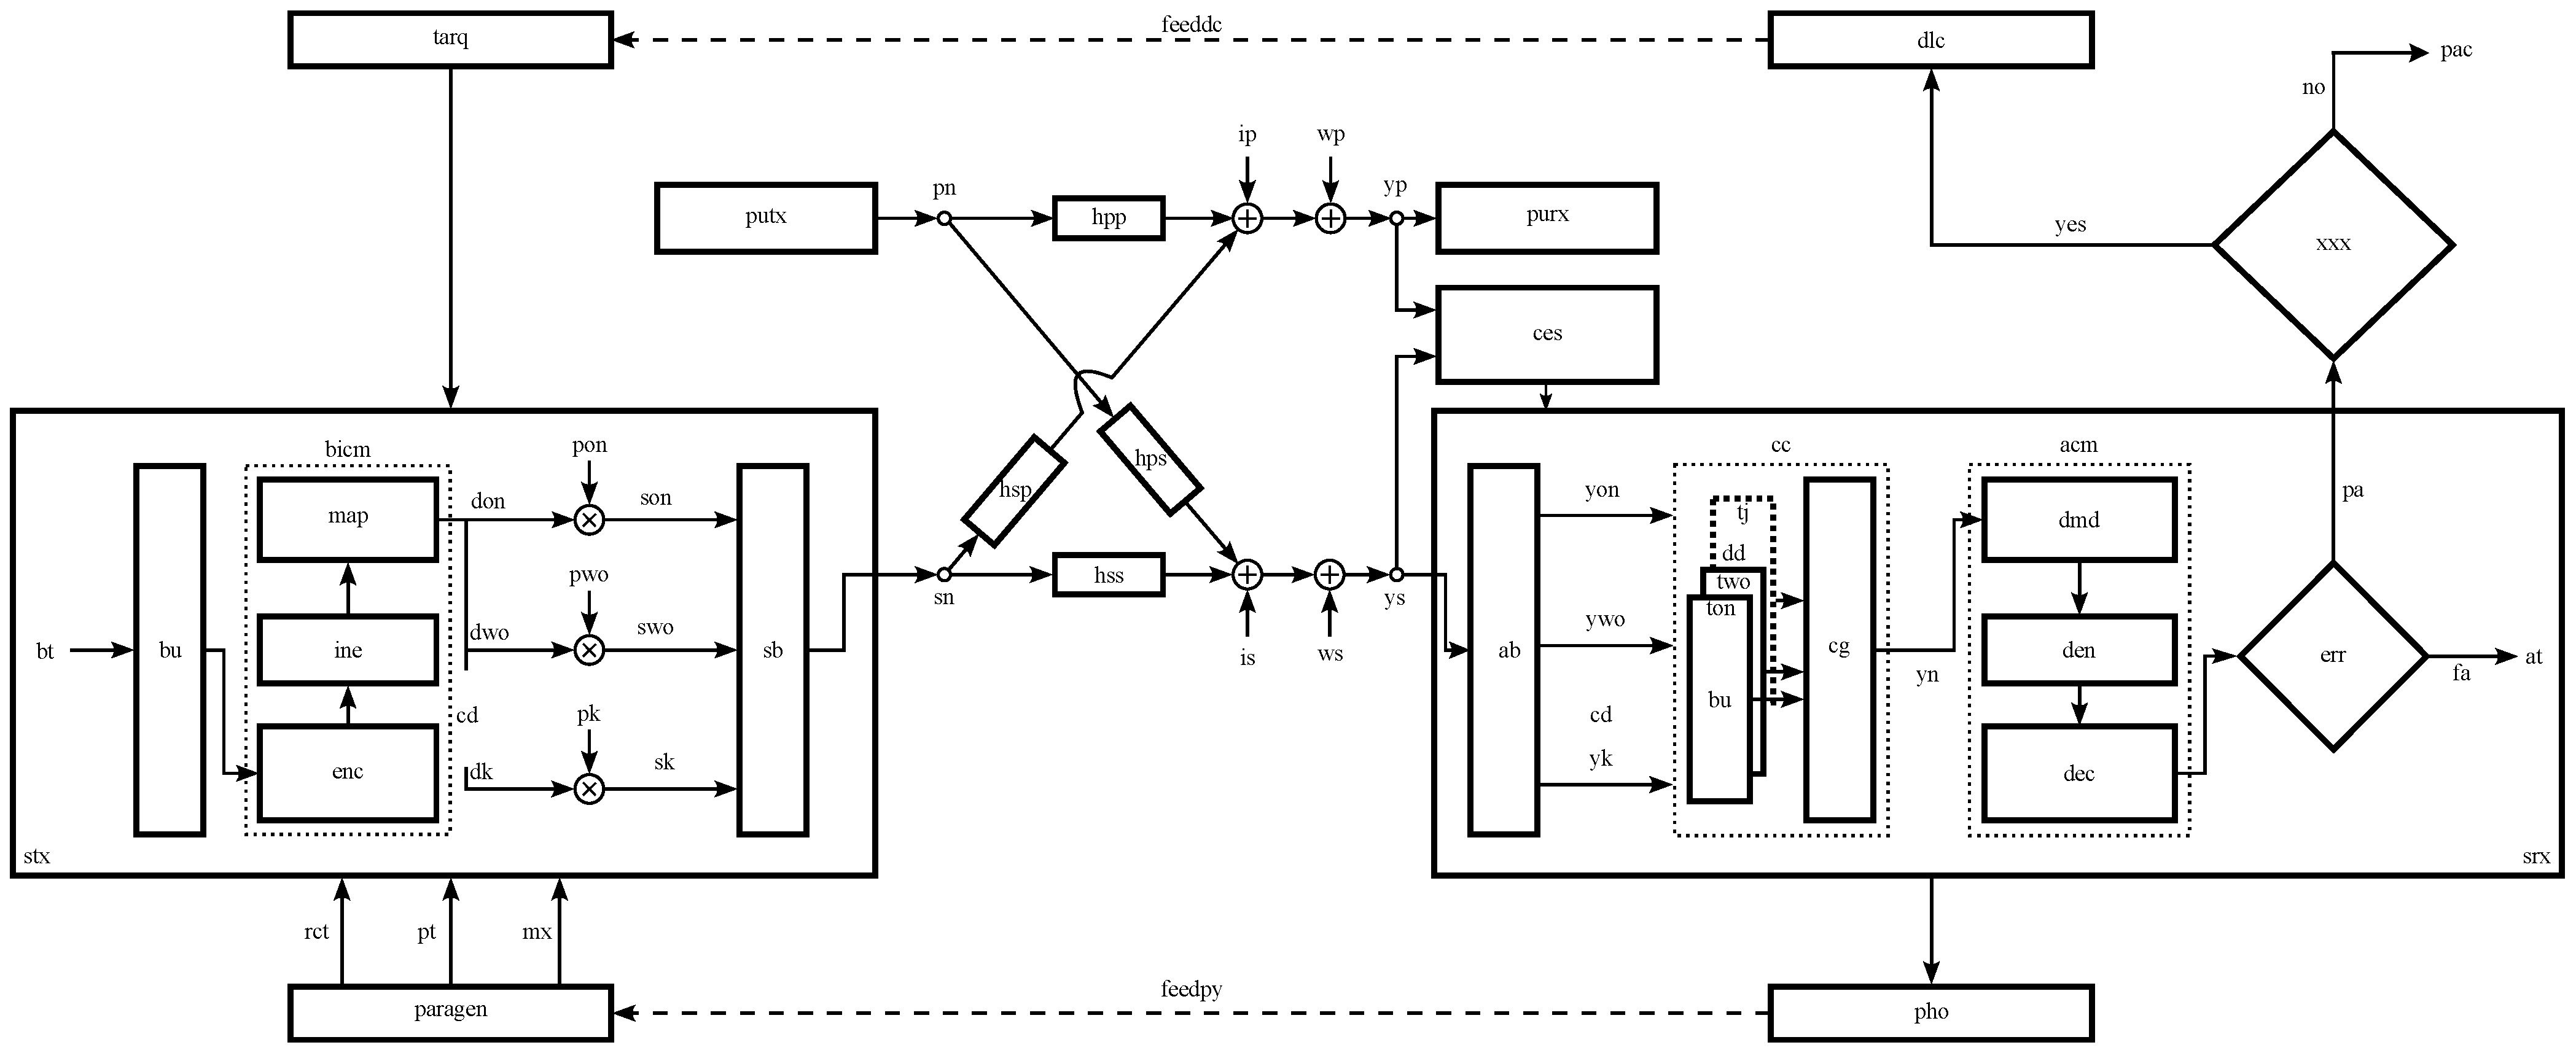
\includegraphics[width=\textwidth]{Figures/findraw_240101.eps}
  \end{psfrags}
  \caption{{\normalsize Underlay CR system model with cross-layer optimization and chase combining.}}
  \label{fig:1}
\end{figure*}

All these methods, however, do not consider any collective adaptation of coding and modulation schemes along with a \myCC{} implementation. The authors in \cite{Mansour2022_alt} propose a \myCLO{} of \myUCRS{} with a discrete Fourier transform modulated filter bank (\myDFTFB{}) using joint bit loading (\myBL{}) and power loading (\myPL)~(\myJBPL) coupled with coding adaptation (\myCA) and \myTHARQ{}. They employ bit-interleaving in combination with minimization of the uncoded bit-error-rate, which allows using different channel coding schemes to minimize coded bit-error-rate. A stochastic chance-constrained programming (\mySCP{}) \cite{Ding2012_alt} is applied to satisfy an interference constraint at the \myPU{} \myRX{} with a given confidence level.

In this paper, the work in~\cite{Mansour2022_alt} is extended as follows:
\vspace{0.5em}
\begin{itemize}[leftmargin=0.9em]
    \renewcommand\labelitemi{$\scriptstyle\bullet$}
    \item In \cite{Mansour2022_alt}, a \myTHARQ{} type \myI{} is considered where erroneous packets are discarded and no diversity or combination gains can be achieved, degrading the achievable \mySE{}. In this paper, a \myTHARQ{} type \myII{} operation with \myCC{} is considered to exploit diversity and combination gains to maximize the achievable \mySE{}.
    \item In~\cite{Mansour2022_alt}, convolutional coding is used in combination with puncturing, while in this paper an \myLDPC{} coding transmission is considered in combination with rate matching, providing better error-correction performance and lower error floors.
    \item The closed form of the lower bound on the \mySE{} in \cite{Mansour2022_alt} is extended and maximized considering \myLDPC{} coding and \myCC{} protocols subject to specific \myQoS{} and interference constraints, validated numerically.
\end{itemize}
\vspace{0.5em}

This paper is organized as follows. Sect.~\ref{sec:2} describes the \myUCRS{} with the \myDFTFB{}s using \myCLO{} and \myTHARQ{} under the influence of third-party interference (\myTPI{}) in addition to the \myPU{} signal. In Sect.~\ref{sec:3}, the \myCLO{} for coded \mySU{} transmission is presented with physical layer (\myPHY{}) and data link control layer (\myDLC{}) parameters. The \myCLO{} system performance is evaluated in Sect.~\ref{sec:4}. Conclusions are drawn in Sect.~\ref{sec:5}.

In this paper, vectors are represented by boldfaced characters and random variables (\myRV s) by capital letters. Furthermore, $\myE{\cdot}$, $\EX{X}{\cdot}$, $\inner{\cdot}{\cdot}$, and $\cond{X}{Y}{y}$ denote expectation, expectation with respect to the \myRV{} $\myX$, inner product, and an \myRV{} $\myX$ conditioned on the \myRV{} $\myY$ taking a value $\myY = \myy$, respectively. Parameters indexed by roman characters $\myPrm{}$, $\mySrm$, (\myun{}) and (\myco{}) are associated with the (\myPU{}), (\mySU{}), uncoded and coded transmissions, respectively. Finally, we define an index set $\Omegaset{a}{b}$ for $\mya \in \myZbb{}$ and $\myb \in \myNbb{}$.

\vspace{-0.5cm}
\section{\hspace{-0.5em}System Description}
\label{sec:2}

We consider the complex baseband representation of a \myUCRS{} with simultaneous transmissions of one \myPU{} (upper horizontal channel) and one \mySU{} (lower horizontal channel) over a time-frequency (\myTF{}) selective fading channel and \myTPI{} as shown in Fig.~\ref{fig:1}.

At time index $\kappa$, the information bits $\myB_{\kappa} \in \{-1, 1\}$ at the input of the \mySU{} \myTX{} are fed to an adaptive bit-interleaved coded modulation (\myABICM{}) comprising:
\begin{itemize}
    \item an \myLDPC{} encoder equipped with rate-matching to achieve a desired code rate $\myR_{\myc}$,
    \item a bit-wise interleaver providing a total of $\myL \myMtot$ interleaved coded bits $\myBlk \in \{-1, 1\}$ at time slot $\myell$ and subcarrier $k \in \Omega_{0,K}$, and
    \item a \myQAM{} modulator.
\end{itemize}

Here, $L \in \myNbb$ is the number of multicarrier symbols per \myPHY{} packet, with each symbol containing $\myMtot$ bits. Each symbol is mapped to $\myK$ \myQAM{} symbols, where $\myK \in \myNbb$ denotes the number of subcarriers available at the \mySU{} \myTX{}.

In the \myPHY{} (lower feedback channel), the \myCLO{} comprises three steps~\cite{Muttath2022_alt}:

\begin{enumerate}
    \item \textbf{\myCA{}}: An optimized code rate $\myR_{\myc,\myoptrm}$ is selected from the available code rates in $\Omega_{\myRC{}}$ and fed back to the transmitter.
    
    \item \textbf{\myBL{}}: The vector $\mymbf = \big[\mym_0, \ldots, \mym_{\myK-1} \big]^{\myTrm}$, containing the number of bits per subcarrier with $\mym_\myk \in \{2,4,6\}$, is optimized as $\hat{\mymbf}_\myoptrm$ and fed back to the \mySU{} \myTX{}. The bits $\myB_{\ell,\myk}$ are subsequently mapped to a symbol $\myD_{\ell,\myk}$ from a square-lattice \myQAM{} symbol set~\cite{Mansour2022_alt}. Furthermore, a bit-rate constraint is imposed on each symbol:
    \[
        \sum_{\myk \in \Omega_{0,\myK}} \mym_\myk = \myMtot.
    \]
    
    \item \textbf{\myPL{}}: The vector $\mypbf = [\myp_0, \ldots, \myp_{\myK-1}]^{\myTrm}$ is optimized as $\hat{\mypbf}_{\myoptrm}$ and fed back, where $\myp_\myk$ represents the power of the $\myk$th subcarrier signal. The \myQAM{} symbol $\Dlk$ is weighted according to
    \[
        \SSelk = \Dlk \sqrt{\myp_\myk}.
    \]
\end{enumerate}

The signal outputs $\SSelk$ pass through the synthesis \myFB\ (\mySFB{}) to generate the \mySU{} transmit signal
 $\mySSn = \sum\limits_{(\myell,\myk)\in\myZbb\times\myOmegaZeroK}
\mySSellk\mygellk{\myn}$. Here, the \myTF{} shifted pulse $\gkl = \gshift$ of the pulse $\myg[\myn]$ is chosen as to render the analysis \myFB{} (\myAFB{}) output signals mutually orthogonal \cite{Mansour2018_alt}. Furthermore, the \mySU\ \myRX\ uses a \myTHARQ{} type~\myII{} with \myCC{}, which on erroneous reception of the \myCC{} output signal, requests the \mySU\ \myTX\
to retransmit the information. This retransmission cycle goes on for a random number of $\myJ$ transmissions until an error–free transmission
is obtained at the \myCC{} output or the predefined maximum number of
retransmissions $\Jmax$ is exceeded, upon which the packet is deemed lost. The \mySU\ \myRX\ received signals at the output of the \myAFB{} for the $\myj$th
transmission with $j \in \Omega_{1,\Jmax+1}$ are described in the \myTF\
plane by the coefficients.
\vspace{-0.6em}
\begin{align*}
    \hspace{-1.2ex} \YSelkj 
    &= \bigl\langle \myY_{\myS,\myj}, \myg_{\ell,\myk} \bigr\rangle \\
    &= \sum_{\myn \in \myZbb} \YSjn \, \myg^{*}[\myn-\myK \ell] \, 
       e^{ -\myj \frac{2\pi}{\myK} \myn \myk} \\
    &\hspace{-0.7cm}= \HSSelkj \myS_{\mySrm,\ell,\myK,\myj} + \XPSelkj + \ISelkj + \WSelkj
\end{align*}
\vspace{-1.25em}

Here, $\XPSelkj$, $\ISelkj$ and $\WSelkj$ represent the interference caused by the \myPU\ transmission at the \mySU\ \myRX\, zero–mean complex colored Gaussian \myTPI\ and additive white Gaussian noise at the \mySU\ \myRX{}, respectively. The linear channel $\myHcal_{\mySrm\mySrm}$ between the \mySU\ \myTX\ and \mySU\ \myRX\ is modelled as a memoryless wide–sense stationary (\myWSS{}) uncorrelated scattering (\myUS{}) Rayleigh fading channel with \myTF\ channel coefficient $\HSSelkj$, rendering the transmissions independent of one another. A corresponding representation of the\! \myPU{}\! transmit and receive signals along with a complete description of all signals in Fig.~\ref{fig:1} can be found in \cite{Mansour2018_alt}.

\newpage 

The \myAFB{} output signals $\YSelkj$ are \!fed to \!the \myCC\ for equal-gain combining (\myEGC{}), where all received signals $1,\dots,\myj$ of that particular packet are stored in buffers, if any. The combined signal $\YSjelk$ at the output of the \myCC\ is given by
\begin{equation}
  \YSjelk
  = \frac{1}{%
      \sqrt{%
        \sum\limits_{{\myj}'=1}^{\myj} \bigl|\myH_{\mySrm\mySrm,\myk,{\myj}'}\bigr|^{2}%
      }%
    }
    \sum_{{\myj}'=1}^{\myj} \HSSelkjpconj \, \YSelkjp \, .
  \label{eq:1}
\end{equation}


In Fig.~\ref{fig:1}, the combiner output is fed to the block $\myABICMinv$
consisting of a \myQAM\ demodulator, a bit-wise \myDeinterleaver\ and
an \myLDPC\ decoder. The decoded packet is passed to a cyclic
redundancy check~(\myCRC{}) which outputs bit estimates~$\myBhatkhat$~upon passing the \myCRC{} or otherwise signals the next \myTHARQ\ iteration according to Sect.~\ref{sec:3b}.

Depending on the considered application scenario, the channel
estimator at the \mySU{} \myRX{} can be employed for acquisition of channel state information as in~\cite{Su2014_alt} and~\cite{Sharma2017_alt}. For the proposed \myCLO\ scheme, only second-order moments of the considered random channel coefficients are required assumed to be known at the \mySU\ \myTX\ and \mySU\ \myRX{}.


\section{\hspace{-0.5em}SU Cross-Layer Optimization for Coded Transmission}
\label{sec:3}

Here, we present a \myCLO{} approach for the \mySU{} \myLDPC{} coded transmission equipped with \myJBPL{} and \myCA{}. The optimization is considered using \myCC{} subject to \myQoS{} constraints in the presence of a PU transmission, thermal noise, and \myTPI{}. In Sect.~\ref{sec:3A}, we derive an upper bound for the coded \mySU{} bit-error probability (\myBEP{}). This bound is used to define the \mySU{} packet-error probability (\myPEP{}). In Sect.~\ref{sec:3c}, we employ a \myTHARQ{} to maximize a lower bound on the \mySU{} \mySE{}. Subsequently, the time-slot index $\ell$ is dropped as the channel is considered time-invariant.

\subsection{Physical Layer Parameters}
\label{sec:3A}

In~(\ref{eq:1}), we define the random signal-to-noise-plus-interference ratio (\mySINR{}) of the $\myk$th subcarrier of the \mySU{} received signal at the output of the combiner after $\myJ=\myj$ transmissions as
\begin{equation}
\label{eq:2}
\myA^{(\myj)}_{\mySrm,\myk} =
\myp_\myk \, |\myD_\myk|^2 \;
\frac{
    \Bigl[ \sum_{{\myj}'=1}^{\myj} |\myHtilde_{\mySrm\mySrm,\myk,{\myj}'}|^2 \Bigr]^2
}{
    \sum_{{\myj}'=1}^{\myj} |\myHtilde_{\mySrm\mySrm,\myk,{\myj}'}|^2 
    \Bigl( 1 + \myp_{\myPrm} \, |\myHtilde_{\myPrm\mySrm,\myk,{\myj}'}|^2 \Bigr)
}
\end{equation}

Here, $\myp_{\myPrm}$ is the average \myPU{} transmit power per subcarrier and $|\myD_\myk|$ is the magnitude of the \myQAM{} symbol. Also, $\myHtilde_{\mySrm\mySrm,\myk,\myj}$ and $\myHtilde_{\myPrm\mySrm,\myk,\myj}$ represent the normalized \myTF{} channel coefficients between the \mySU{} \myTX{} and \mySU{} \myRX{}, and between the \myPU{} \myTX{} and \mySU{} \myRX{}, respectively, for the $\myk$th subcarrier, where

\begin{align}
\tilde{H}_{\mySrm\mySrm,\myk,\myj} &\coloneqq \frac{H_{\mySrm\mySrm,\myk,\myj}}{\sigma_{\mySrm,\myk}}, 
& \text{where} \;\; \tilde{H}_{\mySrm\mySrm,\myk,\myj} \sim \mathcal{CN}(0,1), \\[0.3em]
\tilde{H}_{\myPrm\mySrm,\myk,\myj} &\coloneqq \frac{H_{\myPrm\mySrm,\myk,\myj}}{\sigma_{\mySrm,\myk}}, 
& \text{where} \;\; \tilde{H}_{\myPrm\mySrm,\myk,\myj} \sim \mathcal{CN}(0,1).
\end{align}

with $\myCcal\myNcal(\mu;\sigma^{2})$ representing a circularly-symmetric complex Gaussian random variable with mean $\mu$ and variance $\sigma^{2}$. 
It is noted that $\bigl|\myHtilde_{\mySrm\mySrm,\myk,\myj}\bigr|^{2}$ and $\bigl|\myHtilde_{\myPrm\mySrm,\myk,\myj}\bigr|^{2}$ follow central chi-square distributions as normalized channel gains, respectively:

\begin{align}
\mathrm{Var}\bigl[\tilde{H}_{\mySrm\mySrm,\myk,\myj}\bigr] 
&= \mathbb{E}\Bigl[ \bigl|\tilde{H}_{\mySrm\mySrm,\myk,\myj}\bigr|^2 \Bigr] 
= \frac{\sigma^2_{\mySrm\mySrm}}{\sigma^2_{\mySrm,\myk}}, \\[0.3em]
\mathrm{Var}\bigl[\tilde{H}_{\myPrm\mySrm,\myk,\myj}\bigr] 
&= \mathbb{E}\Bigl[ \bigl|\tilde{H}_{\myPrm\mySrm,\myk,\myj}\bigr|^2 \Bigr] 
= \frac{\sigma^2_{\myPrm\mySrm}}{\sigma^2_{\mySrm,\myk}}.
\end{align}


Here, $\sigma^{2}_{\mySrm,\myk} = \sigma^{2}_{\mySrm,\myImath,\myk} + \sigma^{2}_{\mySrm,\myW}$ represents the average power of \myTPI{} plus noise at the $\myk$h subcarrier of the \mySU\ \myRX{}.\\ Using the channel gains and after some algebra, the probability density function (\myPDF{}) $\myp_{\myA^{(\myj)}_{\mySrm,\myk}} (\alpha)$ of $A^{(\myj)}_{\mySrm,k}$ in (\ref{eq:4}) conditioned on $\left|\myD_\myk\right| = \myd_\myk$ is defined as
\begin{align}
f^{(\myj)}_{\myA_{\mySrm,\myk}}(\alpha) 
&:= \myu(\alpha) \; 
   \frac{\Gamma(3\myj)}{\Gamma(\myj)^2} 
   \left( \frac{\kappa_\myk}{8} \right)^{\myj/2} 
   \alpha^{\myj/2 - 1} 
   \exp\Bigl(\frac{\kappa_\myk}{8} \, \alpha \Bigr) 
   \nonumber \\[0.2em]
&\quad \times \mathcal{D}_{-3\myj}\Bigl( 2 \sqrt{\frac{\kappa_\myk}{8} \, \alpha} \Bigr),
\label{eq:3}
\end{align}

\noindent with 
\[
\kappa_\myk = \frac{1}{\myp_\myk \, \myd_\myk \, \sigma^2_{\mySrm\mySrm,\myk}}, \quad
\mathcal{D}_\nu(\cdot) \text{ denotes the parabolic cylindrical function~\cite{Gradshteyn2007_alt}}.
\]

and $u(\cdot)$ represents the unit-step function.

To evaluate the system performance, we need the coded \mySU\ transmission \myBEP{}, a closed form representation of which is not available. Instead, we use an upper bound on the expected coded \myBEP{} $\myP^{(\mycorm)}_{\mybrm,\mathrm{\myQAM{}},\myj}$ of the $\myj$th transmission for 
$\myA^{(\myj)}_{\mySrm,\myk} = \alpha^{(\myj)}_{\mySrm,\myk}$ averaged over the statistics of 
$\mathbf{\myA}^{(\myj)}_{\mySrm} = \big[\, \alpha^{(\myj)}_{\mySrm,0},\ldots,\alpha^{(\myj)}_{\mySrm,\myK-1} \,\big]^{\myTrm}$.

Averaging over $\myK$ subcarriers, one obtains

\begin{align}
\myP^{(\mycorm)}_{\mybrm,\myQAMrm,\myj}
&\le \myP^{(\myj)}_{\myUBrm} \notag \\
&\hspace{-1cm}= \sum_{\myd = \myd_{\min}}^{\myn}
   \sum_{\myw = 1}^{\myk}
   \frac{\myw}{\myk}\, \myA_{\myw,\myd}
   \sum_{\nu = 0}^{\lfloor\frac{\myd}{2}\rfloor}
   \binom{\lfloor\frac{\myd}{2}\rfloor}{\nu}
   (-1)^{\nu}\,
   \xi(\nu,\myd,\myj),
\label{eq:4}
\end{align}

with \!$\xi(\nu,\myd,\myj)
=\!\myE[\myAbf{}^{(\myj)}_{\mySrm}]
{
\Bigl(\myP^{(\myunrm)}_{\mybrm,\myQAMrm},\myj\Bigr)^{\lfloor \tfrac{\myd}{2} \rfloor + \nu}
}.$ Here, $\myd_{\myminmathrm}$ and $\myA_{\myw,\myd}$ denote the minimum distance of the parity check matrix corresponding to an $(\myn,\myk)$ \myLDPC\ code, and the number of possible code words of Hamming weight $\myd$ with $\myw$ information bits\linebreak in error, respectively. Furthermore, $\myP^{(\myunrm)}_{\mybrm,\myQAMrm,\myj}$ is the conditional uncoded \mySU\ \myBEP{} of the $\myj$th transmission averaged over $\myK$ subcarriers \cite{Mutti2003_alt}, and is given by
\begin{equation*}
P^{(\myunrm)}_{\mybrm{},\myQAMrm,\myj}
= \frac{1}{3\myMtot}
  \sum_{\myk \in \Omega_{0,\myK}} \beta_{\myk}\,
  \myf\bigl(\alpha^{(\myj)}_{\mySrm,\myk}\bigr)
= \frac{\myG\bigl(\myAbf{}^{(\myj)}_{\mySrm}\bigr)}{3\myMtot}.
\end{equation*}
Here, $\beta_{\myk}= \frac{\sqrt{\myM_{\myk}} - 1}{\sqrt{\myM_{\myk}}}$, with
$\myM_{\myk} = 2^{\mym_{\myk}}$ and the function $
\myf\bigl(\alpha^{(\myj)}_{\mySrm,\myk}\bigr)
=
e^{-\frac{3\alpha^{(\myj)}_{\mySrm,\myk}}{2(\myM_{\myk}-1)}}
+ 3 e^{-\frac{2\alpha^{(\myj)}_{\mySrm,\myk}}{\myM_{\myk}-1}}
$ is the approximation of the Q-function as a sum of two weighted exponential functions~\cite{Mutti2003_alt,Karagiannidis2007_alt}.
The sum of $\myK$ i.i.d. random variables can be expressed as
\[
\mathcal{G}\Bigl(\mathbf{A}^{(\myj)}_{\mySrm}\Bigr) 
= \sum_{k \in \Omega_{0,K}} \beta_k \; 
  f\Bigl(A^{(\myj)}_{\mySrm,k}\Bigr).
\]
\newpage

\begin{minipage}[t][12cm]{\columnwidth}

is approximated as a Gaussian distributed RV
\begin{equation*}
\mathcal{G}\Bigl(\mathbf{A}^{(\myj)}_{\mySrm}\Bigr) \sim 
\mathcal{N}\Bigl( \mu_{\mathcal{G},\myj}, \; \sigma^2_{\mathcal{G},\myj} \Bigr),
\end{equation*}

\noindent
where
\begin{equation*}
\mu_{\mathcal{G},\myj} = \sum_{k \in \Omega_{0,K}} \mu_{k,\myj}, 
\quad \text{and} \quad
\sigma^2_{\mathcal{G},\myj} = \sum_{k \in \Omega_{0,K}} \sigma^2_{k,\myj}.
\end{equation*}

Here, the mean and variance for subcarrier $k$, i.e., $\mu_{k,\myj}$ and $\sigma^2_{k,\myj}$, 
are computed by averaging 
$\beta_k f\bigl(A^{(\myj)}_{\mySrm,k}\bigr)$ 
over the joint statistics of $A^{(\myj)}_{\mySrm,k}$ and the QAM symbol power $|D_k|^2$, 
where $|D_k|^2 = \epsilon$ has the probability mass function~\cite{Mansour2018_alt}:

\begin{equation}
p_{|D_k|^2}(\epsilon)
=
\sum_{i=1}^{K_{m_k}} S_{i,m_k} \;
\delta\Bigl(\epsilon - d^2_{i,m_k} \Bigr),
\label{eq:5}
\end{equation}

with 
$K_{m_k} = 3 - 2 m_k + \frac{m_k^2}{2}$ 
distinct power levels $|D_k|^2 = d^2_{i,m_k}$ in a single quadrant of $\Omega_{\myQAMrm}$.  
The sets $\{ d^2_{i,m_k} \} \subset \Omega_{d,m_k}$ 
and $\{ S_{i,m_k} \} \subset \Omega_{S,m_k}$ are given in~\cite{Ding2012_alt}.  

Using (\ref{eq:3}) and (\ref{eq:5}), the mean can be written as

\begin{equation*}
\begin{split}
\mu_{k,\myj} 
&= \mathbb{E}\bigl[ \beta_k f(A^{(\myj)}_{\mySrm,k}) \bigr] 
= \beta_k \int_0^{\infty} f(\alpha) \, p_{A^{(\myj)}_{\mySrm,k}}(\alpha) \, d\alpha \\[0.2em]
&= \beta_k \frac{\Gamma(3\myj)}{\Gamma(\myj)^2} 
  \sum_{i=1}^{K_{m_k}} S_{i,m_k} 
  \Bigl( \frac{\kappa_{k,i}}{8} \Bigr)^{\myj/2} 
  \int_0^{\infty} 
    \alpha^{\myj/2-1} \,
    \mathcal{D}_{-3\myj}\Bigl( 2 \sqrt{\frac{\kappa_{k,i} \alpha}{8}} \Bigr) 
    e^{\kappa_{k,i}\alpha/8} \\ 
&\quad \times \Bigl( e^{-c_{1,k} \alpha} + 3 \, e^{-c_{2,k} \alpha} \Bigr) 
\, d\alpha \\[0.2em]
&= \beta_k \, \theta_{\myj} 
  \sum_{i=1}^{K_{m_k}} S_{i,m_k} 
  \Bigl( \frac{\kappa_{k,i}}{8} \Bigr)^{\myj/2} 
  \Bigl( \Psi(c_{1,k},\myj) + 3 \, \Psi(c_{2,k},\myj) \Bigr).
\end{split}
\end{equation*}

Here, the function $\Psi(x,\myj)$ is defined as
\[
\Psi(x,\myj) = x^{-\myj/2} \;
\mathcal{F}\Bigl( \tfrac{3\myj}{2}, \tfrac{\myj}{2}; 2\myj + \tfrac{1}{2}; 1 - \tfrac{\kappa_{k,i}}{4x} \Bigr),
\]
where $\mathcal{F}(a,b;c;z)$ denotes the hypergeometric function~\cite{Gradshteyn2007_alt}, 
and 
\[
\kappa_{k,i} = \frac{1}{p_k \, d^2_{i,m_k} \, \sigma^2_{\mySrm\mySrm,k}}.
\]

The constants are given by
\[
c_{1,k} = \frac{3}{2(M_k-1)}, \quad
c_{2,k} = \frac{2}{M_k-1}, \quad
\theta_{\myj} = 
\frac{\Gamma(3\myj) \, \sqrt{\pi}}{\Gamma(\myj) \, \Gamma\bigl(2\myj + \tfrac{1}{2}\bigr) \, (\sqrt{2})^{5\myj-2}}.
\]

Similarly, the variance for subcarrier $k$ is obtained as
\[
\sigma^2_{k,\myj} = 
\mathbb{E}\Bigl[ \bigl( \beta_k f(A^{(\myj)}_{\mySrm,k}) \bigr)^2 \Bigr] - \mu^2_{k,\myj}.
\]
can be found using

\begin{equation*}
\hspace*{-1cm}
\myE[\myA^{(\myj)}_{\mySrm,\myk}]
{
   \left(\myf\left(\myA^{(\myj)}_{\mySrm,\myk}\right)\right)^2
}
= \theta_\myj \sum_{\myi=1}^{\myK_{\mym_\myk}}
\myS_{\myi,\mym_\myk}
\left(\frac{\kappa_{\myk,\myi}}{8}\right)^{\frac{\myj}{2}}
\end{equation*}

\begin{equation*}
\hspace*{0.5cm}
\times\quad \left(
   \Psi(\myc_{3,\myk}, \myj)
   + 9\Psi(\myc_{4,\myk}, \myj)
   + 6\Psi(\myc_{5,\myk}, \myj)
\right),
\end{equation*}

where
$
\myc_{3,\myk} = \frac{3}{\myM_\myk - 1},
\
\myc_{4,\myk} = \frac{4}{\myM_\myk - 1},
\myc_{5,\myk} = \frac{7}{2(\myM_\myk - 1)}.
$

Finally, the upper bound in (\ref{eq:4}) is given by

\begin{equation*}
\begin{aligned}
\myP^{(\myj)}_{\myUBrm}
&=
\sum_{\myd=\myd_{\min}}^{\myn}
\sum_{\myw=1}^{\myk}
\frac{\myw}{\myk}\, \myA_{\myw,\myd}
\sum_{\nu=0}^{\lfloor \frac{\myd}{2} \rfloor}
\binom{\lfloor \frac{\myd}{2} \rfloor}{\nu}
(-1)^{\nu}
\\[4pt]
&\hspace{0.5cm}\times
\left( \frac{1}{3\myMtot} \right)^{\myp}
\sum_{\myi=0}^{\myp}
\binom{\myp}{\myi}\,
\mu^{\myi}_{\myG,\myj}\,
\zeta_{\myp-\myi,\myj},
\end{aligned}
\end{equation*}

\end{minipage}

\newpage
\begin{minipage}[t][12cm]{\columnwidth}

with $\myp = \lfloor \frac{\myd}{2} \rfloor +\nu$ and the central moments for $\myp \in \myNbb$ given by
\begin{align*}
\zeta_{\myp,\myj}
&=
\quad\myE[\myAbf^{(\myj)}_{\mySrm}]
{
    \left(
        \myG\left( \myAbf^{(\myj)}_{\mySrm} \right)
        - \mu_{\myG,\myj}
    \right)^{\myp}
}
\\
&=\quad
1 \cdot 3 \cdot \ldots (\myp-1)\,
\sigma_{\myG,\myj}^{\,\myp}\,
( (\myp+1)\bmod\!2 ).
\end{align*}
The dependeny of the different expressions on $\myR_\myc,$ $\mypbf$ and $\mymbf$ \!is not indicated for better readability of the resulting formulas.
\vspace{-1em}
\subsection{Data Link Layer Parameters}
\label{sec:3b}

The \mySU{} \myRX{} determines if at least one estimated bit $\hat \myB_{\kappa}$ in the received packet is in error compared to the information bit
$B_{\kappa}$, and generates a \myTHARQ{} over a one-bit feedback channel
to request the \mySU{} \myTX{} to retransmit the packet. The \mySU{} \myTX{}
\myTHARQ{} determines and retransmits the required packet from
the \myTX{} buffer. The \myPEP{} $\myP^{(\myj)}_{\mypac}$ of the \mySU{} transmission after $\myj$ transmissions can be upper bounded by a union bound $\myP^{(\myj)}$ given by
\[
\myP^{(\myj)}_{\mypacrm}
= 
\Pr\left\{
    \bigcup_{\kappa = 1}^{\myL \myMtot\myR_{\myc}}
    \; \myB_{\kappa} \ne \hat{\myB}_{\kappa}
\right\}
\le
\myL \myMtot \myR_{\myc} \, \myP^{(\myj)}_{\myUBrm}
= 
\myP^{(\myj)} ,
\]
with 
$\myP^{(\myj)} = \myP^{(\myj)}(\mypbf, \mymbf, \myR_{\myc})$.
To simplify the system analysis,
the following assumptions have been made:
\begin{itemize}[leftmargin=1.9em]
    \renewcommand\labelitemi{$\scriptstyle\bullet$}
    \item A packet is deemed lost, if it is still decoded with errors after $\myJ_{\max}+1$ transmissions.
    \item The noise and \myTPI\ profiles are known at the \mySU\ \myRX\ and \myPU\ \myRX{}.
    \item Perfect error detection is achieved using \myCRC{}.
    \item The feedback channel is error-free and has no latency.
\end{itemize}
To evaluate the system performance of the \mySU\ transmission,
the average \mySU\ \mySE\ is defined by
\begin{equation}
\bar{\myS}(\mypbf,\mymbf,\myR_\myc)
  = \frac{\myL \myMtot \myR_\myc}{\myK}
    \, \myE{\frac{\myImath(\myJ)}{\myJ}},
\label{eq:6}
\end{equation}
with the indicator function
\[
\myImath(\myj) =
\begin{cases}
  1, & \text{for\quad} 1 \le \myj \le \myJ_{\max}+1 \\[0.3em]
  0, & \text{else}.
\end{cases}
\]
Furthermore, the probability for a packet to require $\myj$ transmissions for error-free reception is given by
\begin{equation}
\Pr\{\myj\} =
\begin{cases}
\displaystyle \Bigl( 1 - \myP_{\mypacrm}^{(\myj)} \Bigr) 
\prod_{i=1}^{\myj-1} \myP_{\mypacrm}^{(i)}, 
& 1 \le \myj \le \myJ_{\max}, \\[1em]
\displaystyle \prod_{i=1}^{\myj-1} \myP_{\mypacrm}^{(i)}, 
& \myj = \myJ_{\max}+1.
\end{cases}
\label{eq:7}
\end{equation}

\noindent
Using (\ref{eq:6}) and (\ref{eq:7}), a lower bound on the spectral efficiency can be written as
\[
\myS_{\myLBrm} \le \bar{\myS}(\mypbf,\mymbf,\myR_\myc),
\]
where
\begin{equation}
\myS_{\myLBrm} 
= \alpha \, \mathbb{E} \Biggl[
    \frac{\myI(\myJ)}{\myJ} \;\Big|\; \myP_{\mypacrm}^{(\myj)} \to \myP^{(\myj)}
\Biggr]
= \alpha \left(
    1 - \sum_{\myj=1}^{\myJ_{\max}} 
        \frac{\displaystyle \prod_{i=1}^{\myj-1} \myP^{(i)}}{\myj (\myj+1)}
\right).
\label{eq:8}
\end{equation}

with $\alpha = \frac{\myL \myMtot \myR_{\myc}}{\myK}$. 
Similarly, an upper bound $\bar{\myJ}_{\myUBrm}$ on the
average number of transmissions $\bar{\myJ}$ is given by
\begin{equation*}
    \bar{\myJ}_{\myUBrm}
    = \myE {\, \myJ \,\big|_{\myP_{\mypacrm}^{(\myj)} \leftarrow \myP^{(\myj)}} }
    = 1 + \sum_{\myj=1}^{\myJ_{\max}} \prod_{\myi=1}^{\myj} \myP^{(\myi)} .
\end{equation*}

\end{minipage}

\clearpage

\subsection{Cross-Layer Optimization Problem}
\label{sec:3c}
\myCLO\ is proposed to maximize $\myS_{\myLBrm}$ in (\ref{eq:8}) by carefully selecting
$(\mypbf, \mymbf, \myR_{\myc}) \in \Omega_{\myp} \times \Omega_{\mym} \times \Omega_{\myR_{\myc}}$
taking into account specific \myQoS\ constraints outlined below. Here, $\Omega_{\myp}$,
$\Omega_{\mym}$ and $\Omega_{\myR_{\myc}}$ represent the set $\myRbb^{+}_{0}$ of powers,
the set of $\myK$-length vectors of possible BL patterns \cite{Mansour2018_alt} and the set of
rate-matched \myLDPC\ code rates available at the \mySU\ \myTX{}. The maximization problem reads
\begin{equation*}
\left[ \hat{\mypbf}_{\myoptrm},\,
       \hat{\mymbf}_{\myoptrm},\,
       \hat{\myR}_{\myc,\myoptrm}
\right]
=\arg\hspace{-4ex}\max\limits_{(\mypbf,\,\mymbf,\,\myR_\myc)\in\Omega_{\mypbf}\times\Omega_{\mymbf}\times\Omega_{\myR_\myc}}
\hspace{-0.5ex}S_{\myLBrm}(\mypbf,\,\mymbf,\,\myR_\myc)
\end{equation*}

\begin{align}\hspace{2.5cm}
    \text{subject to}\qquad\quad 
    \myp_\myk &\ge 0                                   
        && \label{eq:9} \\
    \sum_{\myk\in\Omega_{0,\myk}} \myp_\myk &\le \myp_{\mytotrm}      
        && \label{eq:10} \\
    (\mym_\myk - 2)(\mym_\myk - 4)(\mym_\myk - 6) &= 0            
        && \label{eq:11} \\
    \sum_{\mym_\myk\in\Omega_{0,\myk}} \mym_\myk &= \myMtot      
        && \label{eq:12} \\
    \Pr\{\myI_\myk \le \myi_{\mytemprm}\} &\ge \mya
        && \label{eq:13} \\
    \myD &\le \myD_{\max}                             
        && \label{eq:14} \\
    L\myMtot \myR_\myc &\ge \myM_{\myreqrm} 
        && \label{eq:15} \\
    \prod_{\myj=1}^{\myJ_{\mymax}+1} \myP^{(\myj)} &\le \myp_{\myreqrm}.
        && \label{eq:16}
\end{align}
In~(\ref{eq:9}), the \myCLO{} allocates a non-negative $\myp_\myk$ to each subcarrier,
while adhering to a constraint on the total available \mySU{} \myTX{}
transmit power $\myp_{\mytotrm} \ge 0$ specified in~(\ref{eq:10}). The \myBL\ using the available \myQAM\ orders mentioned in Sect.\myII\ is represented in (\ref{eq:11}) maintaining the bit-rate constraint in~\!(\ref{eq:12}) with \!$\myMtot\!=2\myM$ and a fixed integer value $\myM$ chosen to support the intended
bit-rate with $\myK \le \myM \le 3K$ according to the available bit
patterns in~(\ref{eq:11}). In~(\ref{eq:13}), we ensure that the \mySU{} transmission
interference at the \myPU{} \myRX{} does not exceed a predefined $\myi_{\mytemprm}$
with a confidence level $\mya$. The closed form of the interference
constraint in~(\ref{eq:13}) is calculated similar to~\cite{Mansour2018_alt} according to
\begin{equation*}
\Pr\{\myI_\myk \le \myi_{\mytemprm}\}
    = 1 - \sum_{\myi=1}^{\myK_{\mym_\myk}}
        \psi\!\left(\myS_{\myi,\mym_\myk},\, \myd^{2}_{\myi,\mym_\myk},\, \myp_\myk,\, \myk\right) ,
\end{equation*}
where $\myI_\myk$ is the interference of the non-\myPU\ signal at the \myPU\ \myRX\ at the $\myk$th subcarrier. Furthermore,
{\small
\begin{equation*}
\psi\!\left(\myS, \myd^2, \myp, \myk\right)
= \myS \sqrt{\frac{4\phi_{\myp}}{\myp \sigma_{\mySrm\myPrm}^{2} d^{2}
    + \sigma_{\mathrm{\myP,\myI},\myk}^{2}}}\;
\myK_{1}\!\left(
        \sqrt{\frac{4\phi_{\myp}}{
        \myp \sigma_{\mySrm\myPrm}^{2} \myd^{2}
        + \sigma_{\myPrm,\myImath,\myk}^{2}}}
     \right),
\end{equation*}
}
with
$\phi_{\myp} = \frac{\myi_{\mytemprm}}{\myp\,\sigma_{\myPrm\myPrm}^{2}}$
and $\myK_{1}(\cdot)$ being the first-order modified Bessel function of the second kind.
Here,
$\sigma_{\myPrm\myPrm}^{2}
    = \myE{ \left| \myH_{\myPrm\myPrm,\myk,\myj} \right|^{2} }
\quad\text{and}\quad
\sigma_{\mySrm\myPrm}^{2}
    = \myE{ \left| \myH_{\mySrm\myPrm,\myk,\myj} \right|^{2}}$ are the channel gains between the \myPU\ \myTX\ and \myPU\ \myRX\, and the
\mySU\ \myTX\ and \myPU\ \myRX\, respectively. 
Furthermore, the \myCLO{} ensures that the \mySU{}
transmission satisfies the \myQoS\ constraints in (\ref{eq:14})-(\ref{eq:16}). First, by selecting
$\myJ_{\max} = \left\lfloor \myD_{\max}/\myD_{\mytriprm}\right\rfloor$ where $\myD_{\mytriprm}$ defines the round-trip delay of each
retransmission and $\myD_{\max}$ is the maximum delay, we ensure the total
transmission delay $\myD$ does not exceed $\myD_{\max}$ in (\ref{eq:14}).
Secondly, a suitable \linebreak
\newpage
$\myR_\myc \in \Omega_{\myR_\myc}$ is selected to guarantee a minimum required data
rate $\myM_{\myreqrm}$ in (\ref{eq:15}). Finally, in (\ref{eq:16}), the \myCLO\ ensures that the
\mySU\ \myPEP\ even after $\myJ_{\max}+1$ transmissions does not exceed a predefined threshold $\myp_{\myreqrm}$.




\section{Performance Analysis}
\label{sec:4}
\noindent The system in Fig.~\ref{fig:2} is simulated in \textbf{MATLAB} with 
$K = 64$ subcarriers, $L = 1$ multicarrier symbol per packet, and $\Mtot = 4K$. 
The total available SU TX transmit power is $\ptot = K$. 
Assuming the thermal noises at both the PU RX and SU RX arise from the same type 
of front-end amplifiers, we choose $\sigma_{\mathrm{P},\mathrm{W}}^2 = \sigma_{\mathrm{S},\mathrm{W}}^2$. 
Similarly, as both PU and SU coexist in the same band (e.g., an industrial, scientific and medical band), 
we assume the TPI profiles $\sigma_{\mathrm{P},I,k}^2 = \sigma_{\mathrm{S},I,k}^2$ and 
the average TPI power 
$\frac{1}{K} \sum_{k \in \Omega_{0,K}} \sigma_{\mathrm{S},I,k}^2 = \sigma_{\mathrm{S},\mathrm{W}}^2$. 
The interference temperature is chosen as 
$i_{\mathrm{temp}} = \beta \, \pp \, \sigma_{\mathrm{P}}^2 \, \sigma_{\mathrm{P},\mathrm{W}}^2$ 
with the allowed interference power relative to the thermal noise interference at the PU RX 
to be $\beta = 5$ and a confidence level $a = 0.9$. 
Furthermore, for simplicity, $\sigma_{\mathrm{SP}}^2 = 1/\sigma_{\mathrm{PS}}^2$ and $\pp = \sigma_{\mathrm{S},\mathrm{W}}^2$. 

\begin{figure}[htbp]
\centering
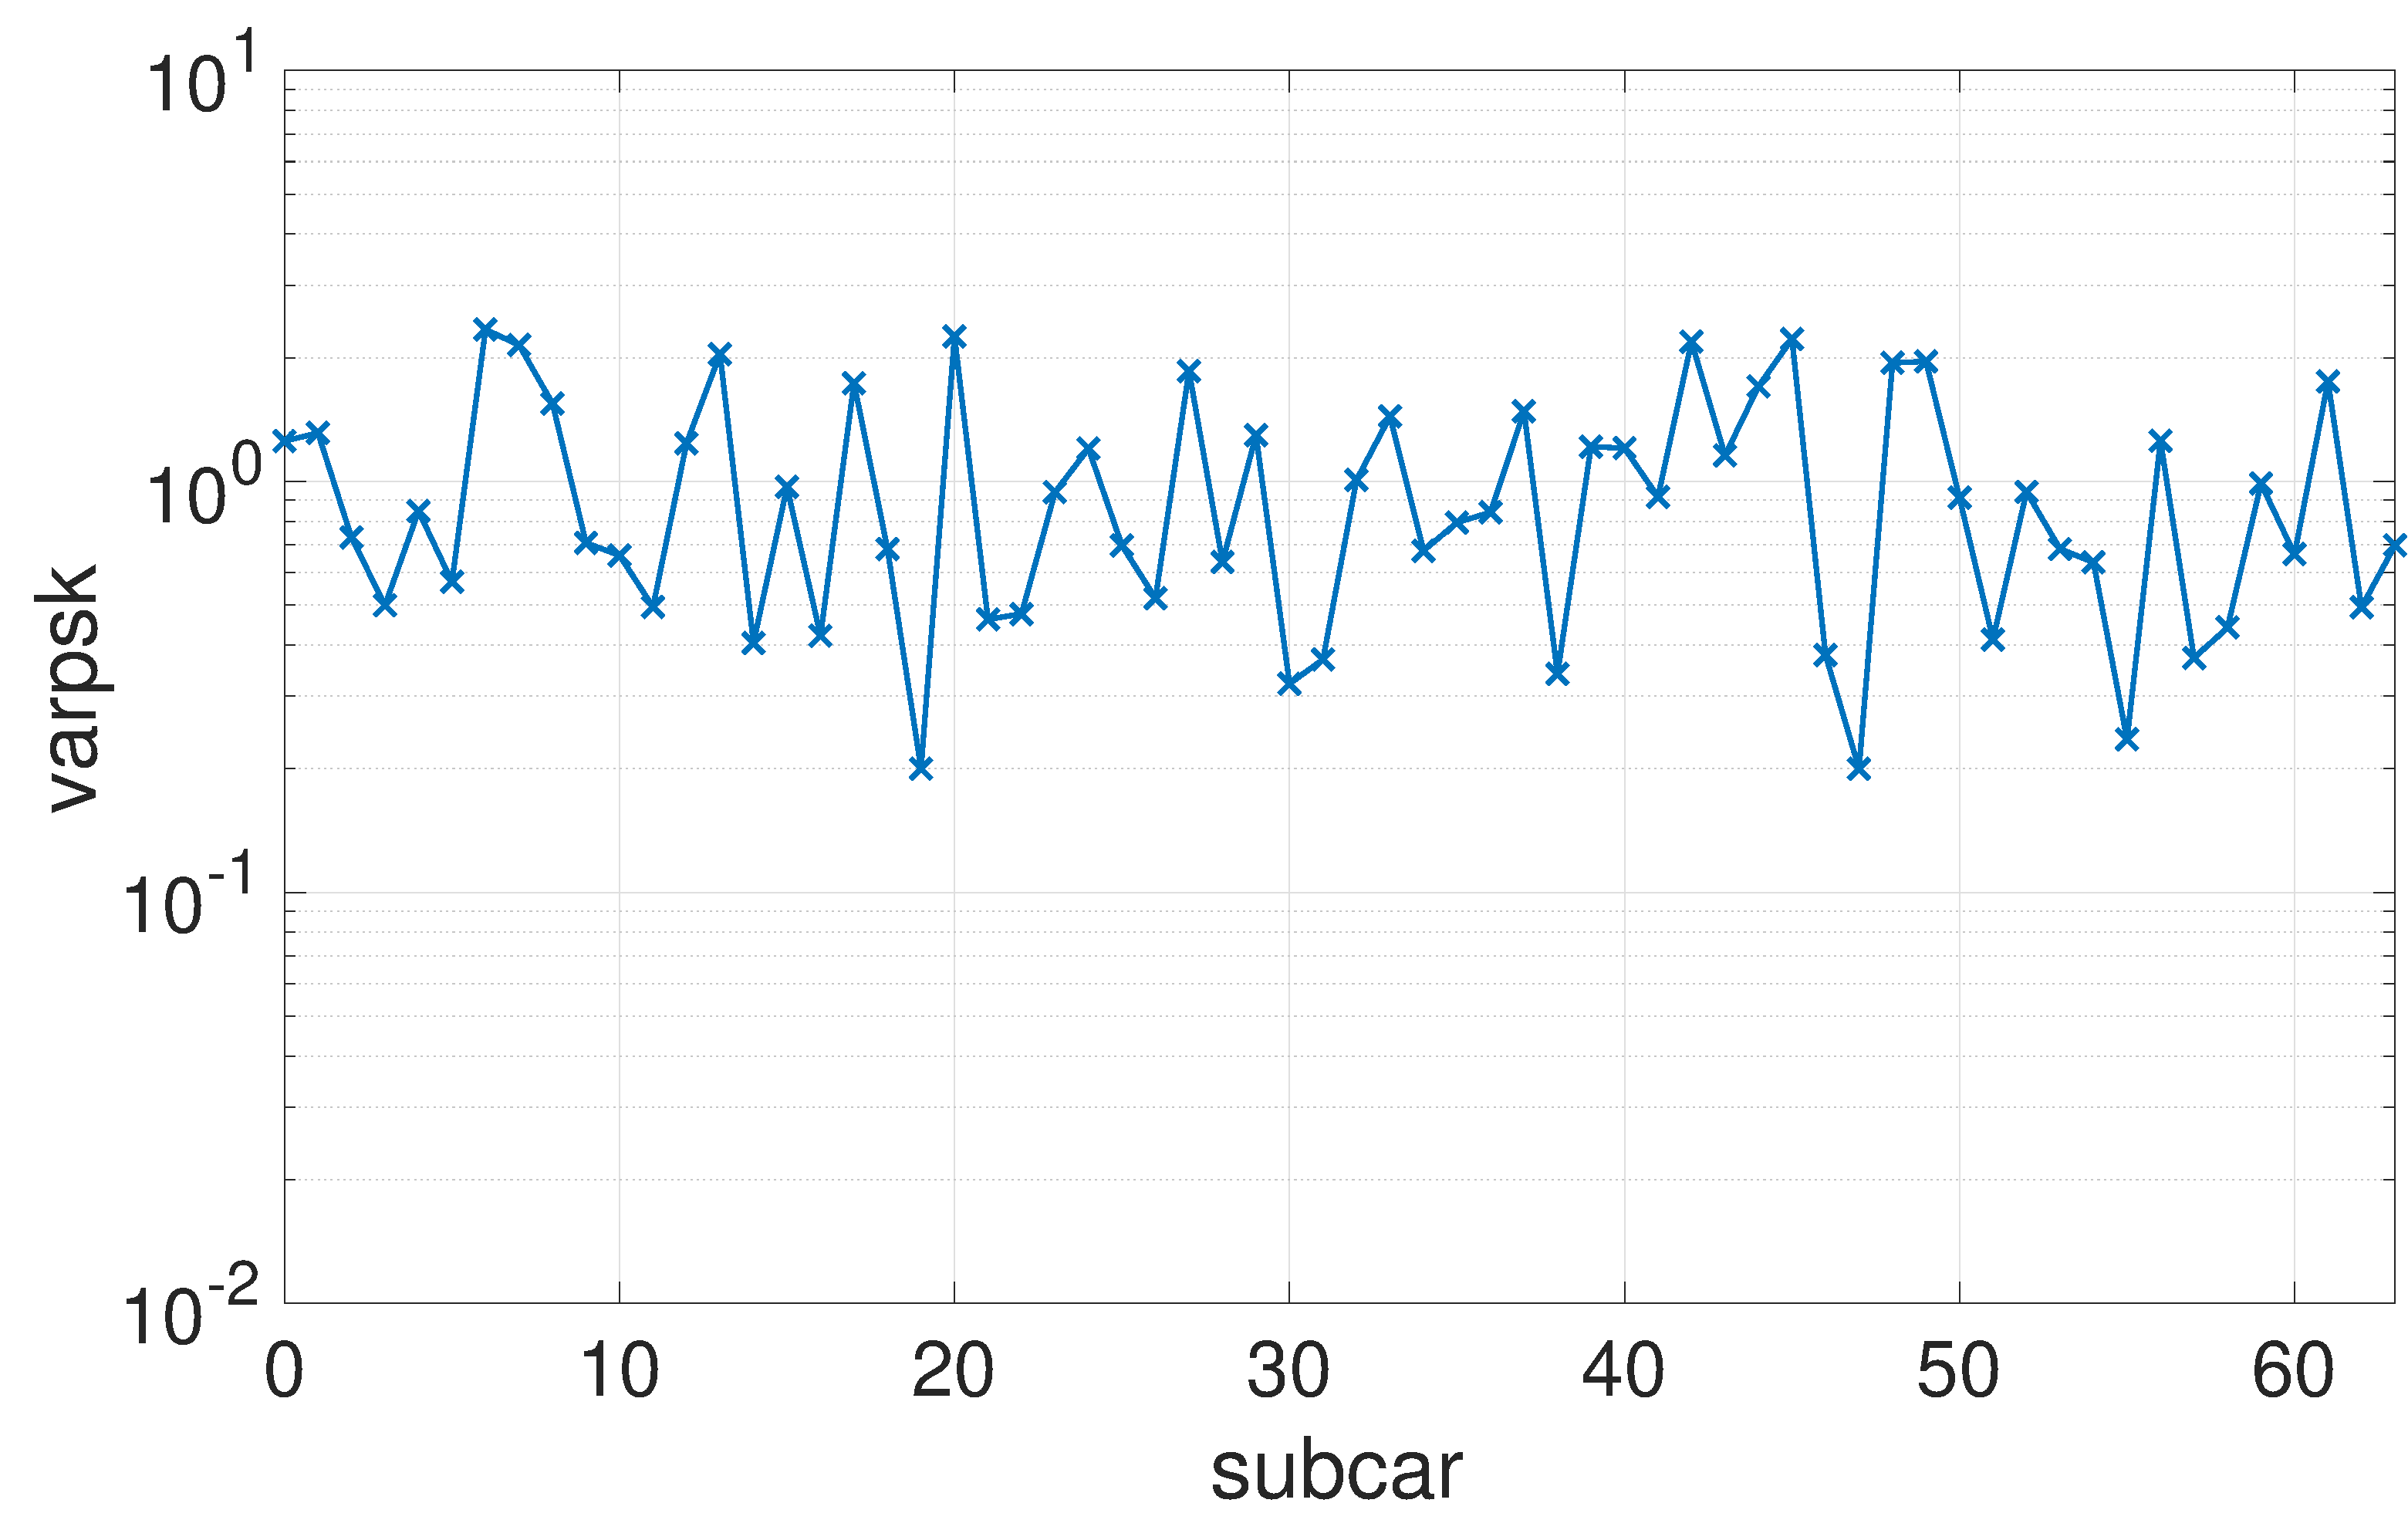
\includegraphics[width=\linewidth]{Figures/varpsk.eps}
\caption{Normalized channel gain profile $\sigma^2_{PS,k}$ between PU TX 
and SU RX.}
\label{fig:2}
\end{figure}

\noindent Moreover, for CA, a rate-matched LDPC encoder is considered. Using the technical specifications in \cite{ETSI2020}, 
a \BGTwo{} parity check matrix is considered with \LiftSize{} and base code rate \(\BaseRate\). 
This code is rate-matched depending on the CA output to give code rates chosen from \(\Omega_{R_c} = \RateSet\). 
The QoS limits are chosen as \(\Mreq = M_{\mathrm{tot}}/3\), \(\Jmax = \JmaxVal\), and \(\preq = \preqVal\). 
Furthermore, Tab.~\ref{tab:ga_params} shows a list of parameters to implement a mixed-integer non-linear optimization problem 
with stochastic chance-based constraints in MATLAB to maximize $\rbSLB$. 
A genetic algorithm (\GA) has been used to exploit its parallel search capability and increase the chance of finding a global optimum to our optimization problem.

\begin{table}[htbp]
\centering
\caption{MATLAB GA parameters for maximization of $\rbSLB$.}
\label{tab:ga_params}
\begin{tabular}{|c|c|} 
\hline
Number of variables & 129 \\
Population size & 500 \\
Max number of generations & 5000 \\
Max number of stall generations & 30 \\
Crossover probability & 0.8 \\
Mutation probability & 0.1 \\
Function tolerance & $1 \times 10^{-6}$ \\
Constraint tolerance & $1 \times 10^{-6}$ \\
Nonlinear constraint solver & penalty \\
Creation function & \texttt{gacreationnonlinearfeasible} \\
\hline
\end{tabular}
\end{table}

For the aforementioned parameters, the CLO performance is
evaluated from the simulated SE values, the optimum code
rates and the number of transmissions required for error-free
transmission as a function of the average energy-per-bit-tonoise
ratio at the SU RX defined by
\begin{equation*}
\eta = \frac{1}{\rbRc \rbsigmaSW^2} \left( \frac{1}{\rbK} \sum_{k \in \rbOmega} \frac{\rbpk \rbsigmaSSk^2}{\rbmk} \right).
\end{equation*}
The CLO is evaluated in the range $\eta \in [0~\text{dB}, \ldots, 40~\text{dB}]$. In Fig.~3, the optimum code rate $\rbRcopt$ selected by the CLO for the cases with and without CC are compared.
\begin{figure}[htbp]
    \centering
    \psfrag{codebest}[c][c]{\scriptsize $\rbRcopt$}
    \psfrag{codenocc}[c][c]{\scriptsize \hspace{2em}$\rbRcopt$-no CC}
    \psfrag{codecc}[c][c]{\scriptsize \hspace{2em}$\rbRcopt$- CC}
    \psfrag{eta}[c][c]{\scriptsize $\rbEtaDB$}
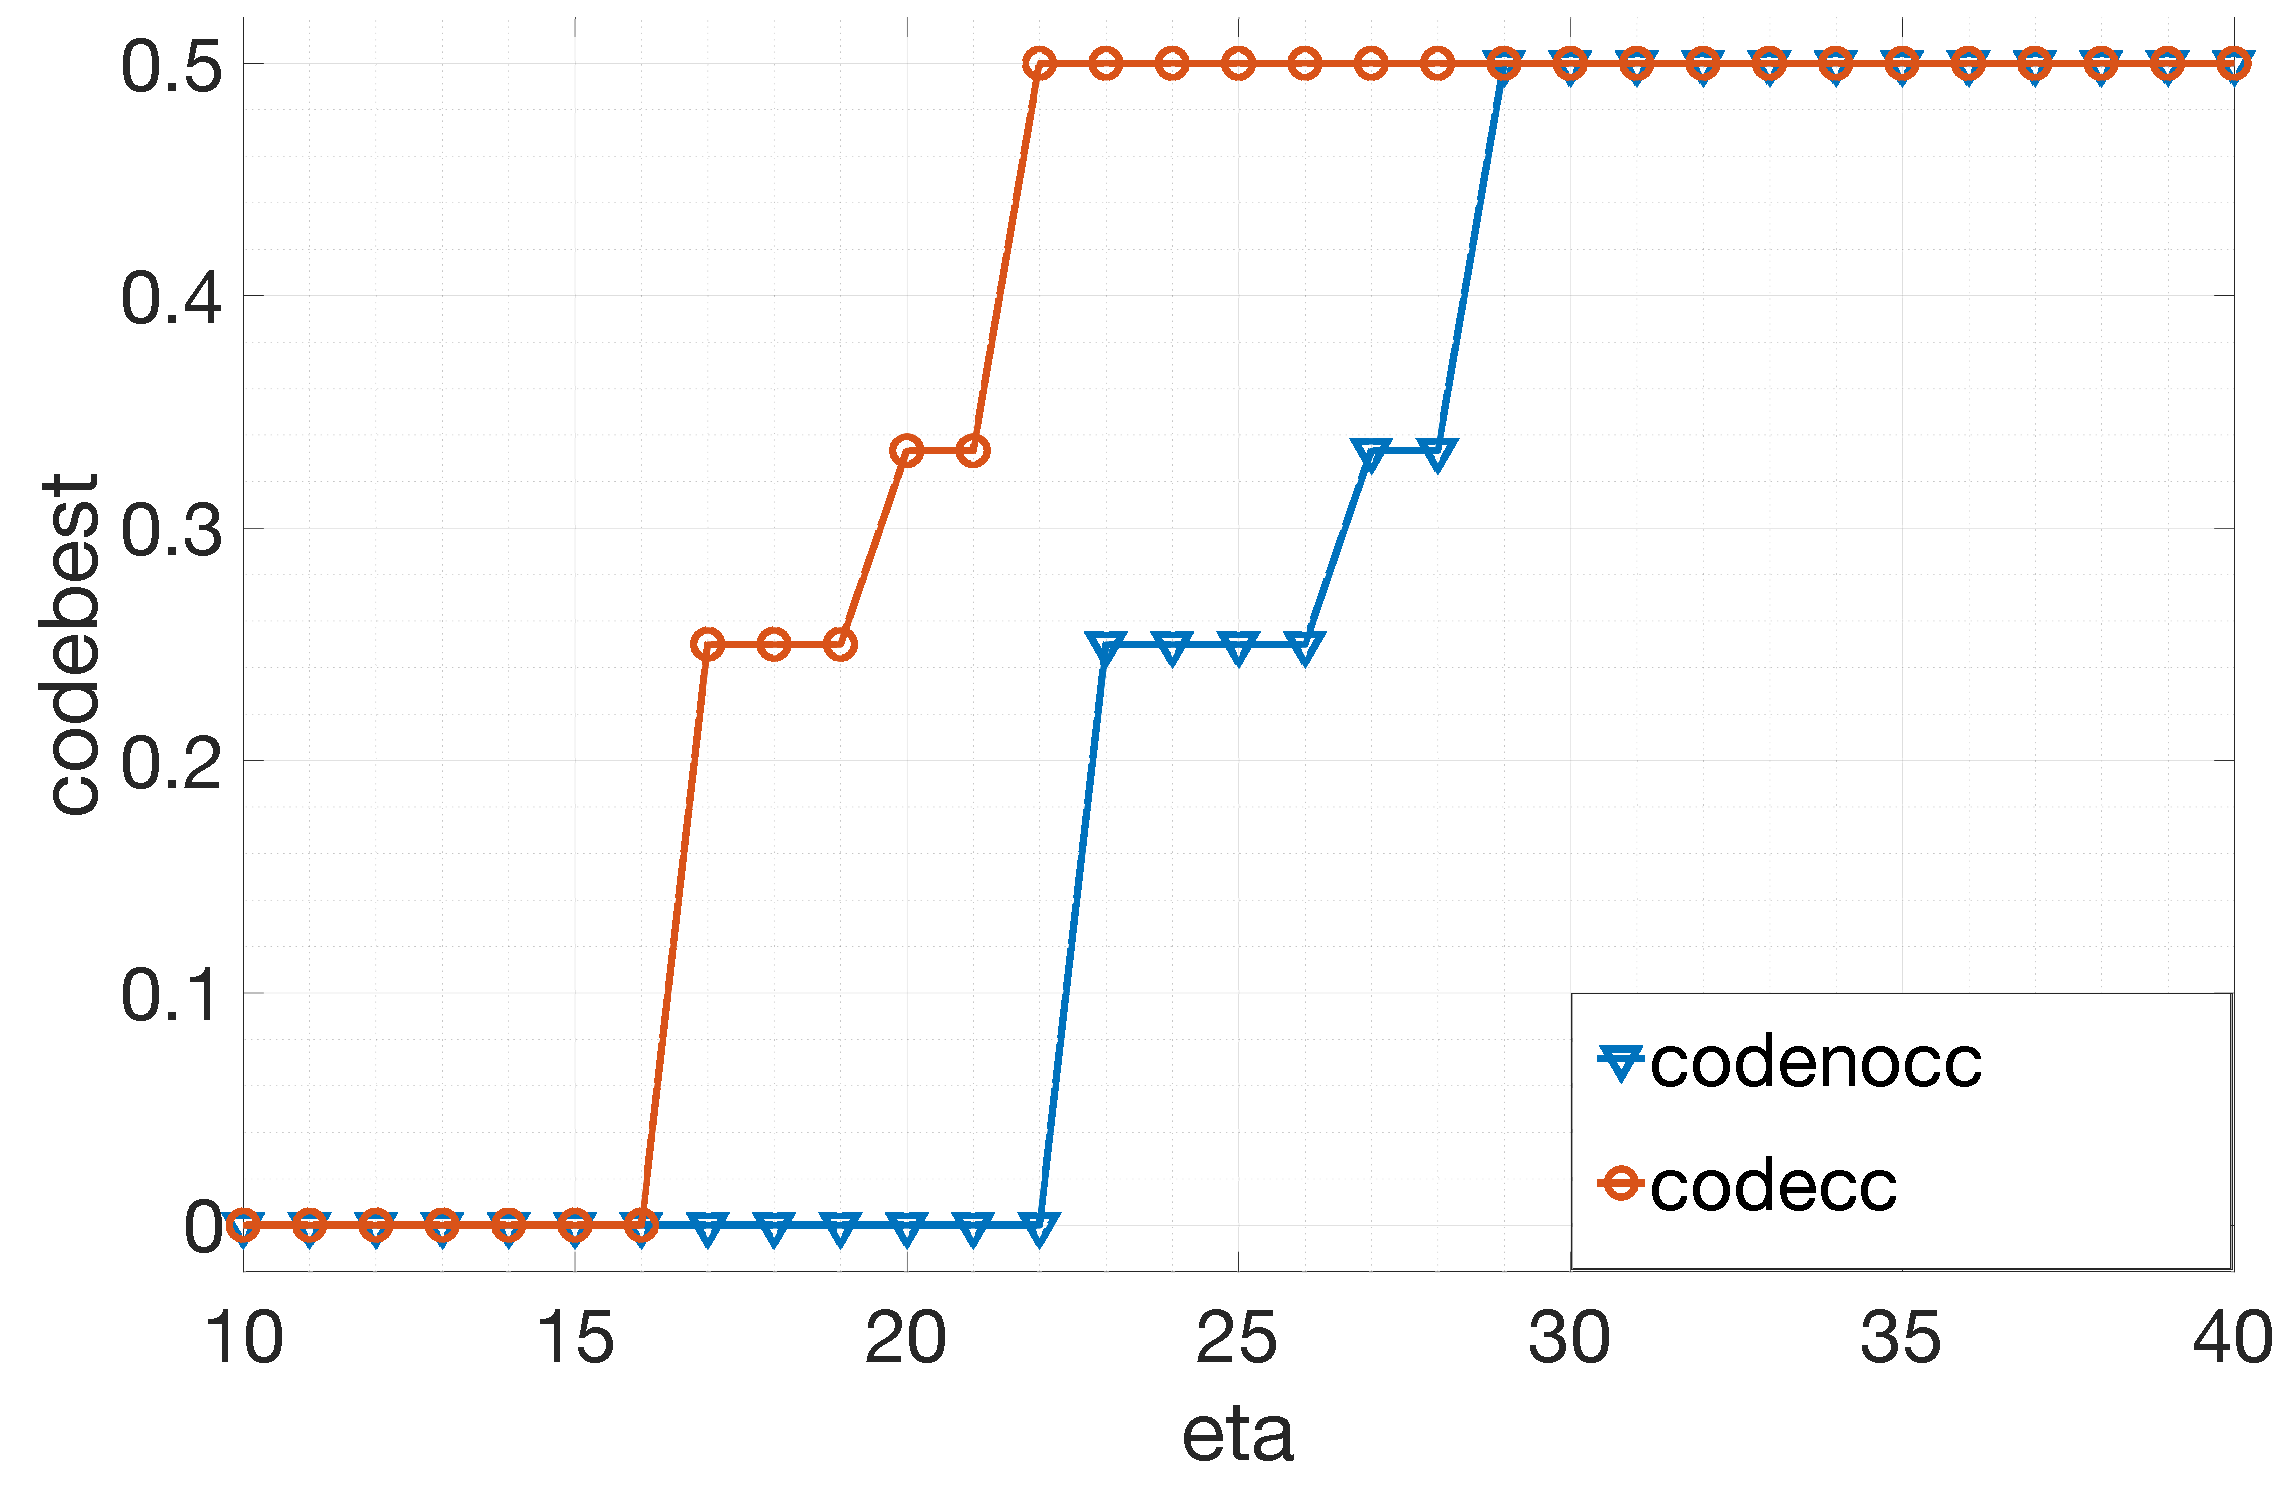
\includegraphics[width=0.8\columnwidth]{Figures/rcscompare_240111.eps}
   \caption{Optimum adaptive coding rate $\hat{R}_{c,\text{opt}}$ versus $\eta$ for $J_{\max} = 2$, $M_{\text{req}} = M_{\text{tot}}/3$, and $p_{\text{req}} = 0.1$.}
    \label{fig:example}
\end{figure}


As can be seen, for the case with (without) CC, the CLO has
no solution up to $17~\text{dB}$ ($23~\text{dB}$), as it, e.g., violates the QoS
constraints in {14} and/or {16}. Clearly, increasing $\eta$ further
allows the CLO to choose higher coding rates from $\rbRc$, where
with CC, one switches to a higher $\rbRcopt$ at smaller $\eta$ compared
to the case without CC.

In Fig.~4, we investigate the gap between the achievable SE $S$
and the lower bound $\rbSLB$ from the CLO for the cases with and
without CC, resp., together with the optimum corresponding
rates $\rbRcopt$ from Fig.~3.

\begin{figure}[htbp]
    \centering
    \psfrag{sslb}[c][c]{\scriptsize $\rbSLB~\rbSLBunit$}         
    \psfrag{slbnocc}[c][c]{\scriptsize\hspace{4em}$\rbSLB~\rbCLOnocc$} 
    \psfrag{slbcc}[c][c]{\scriptsize\hspace{4em} $\rbSLB~\rbCLOcc$} 
    \psfrag{snocc}[c][c]{\scriptsize\hspace{4em} $S~\rbSimnocc$}   
    \psfrag{scc}[c][c]{\scriptsize\hspace{4em} $S~\rbSimcc$} 
    \psfrag{codenocc}[c][c]{\scriptsize \hspace{2em}$\rbRcopt$-no CC}
    \psfrag{codecc}[c][c]{\scriptsize \hspace{2em}$\rbRcopt$- CC}
    \psfrag{eta}[c][c]{\scriptsize $\rbEtaDB$}
    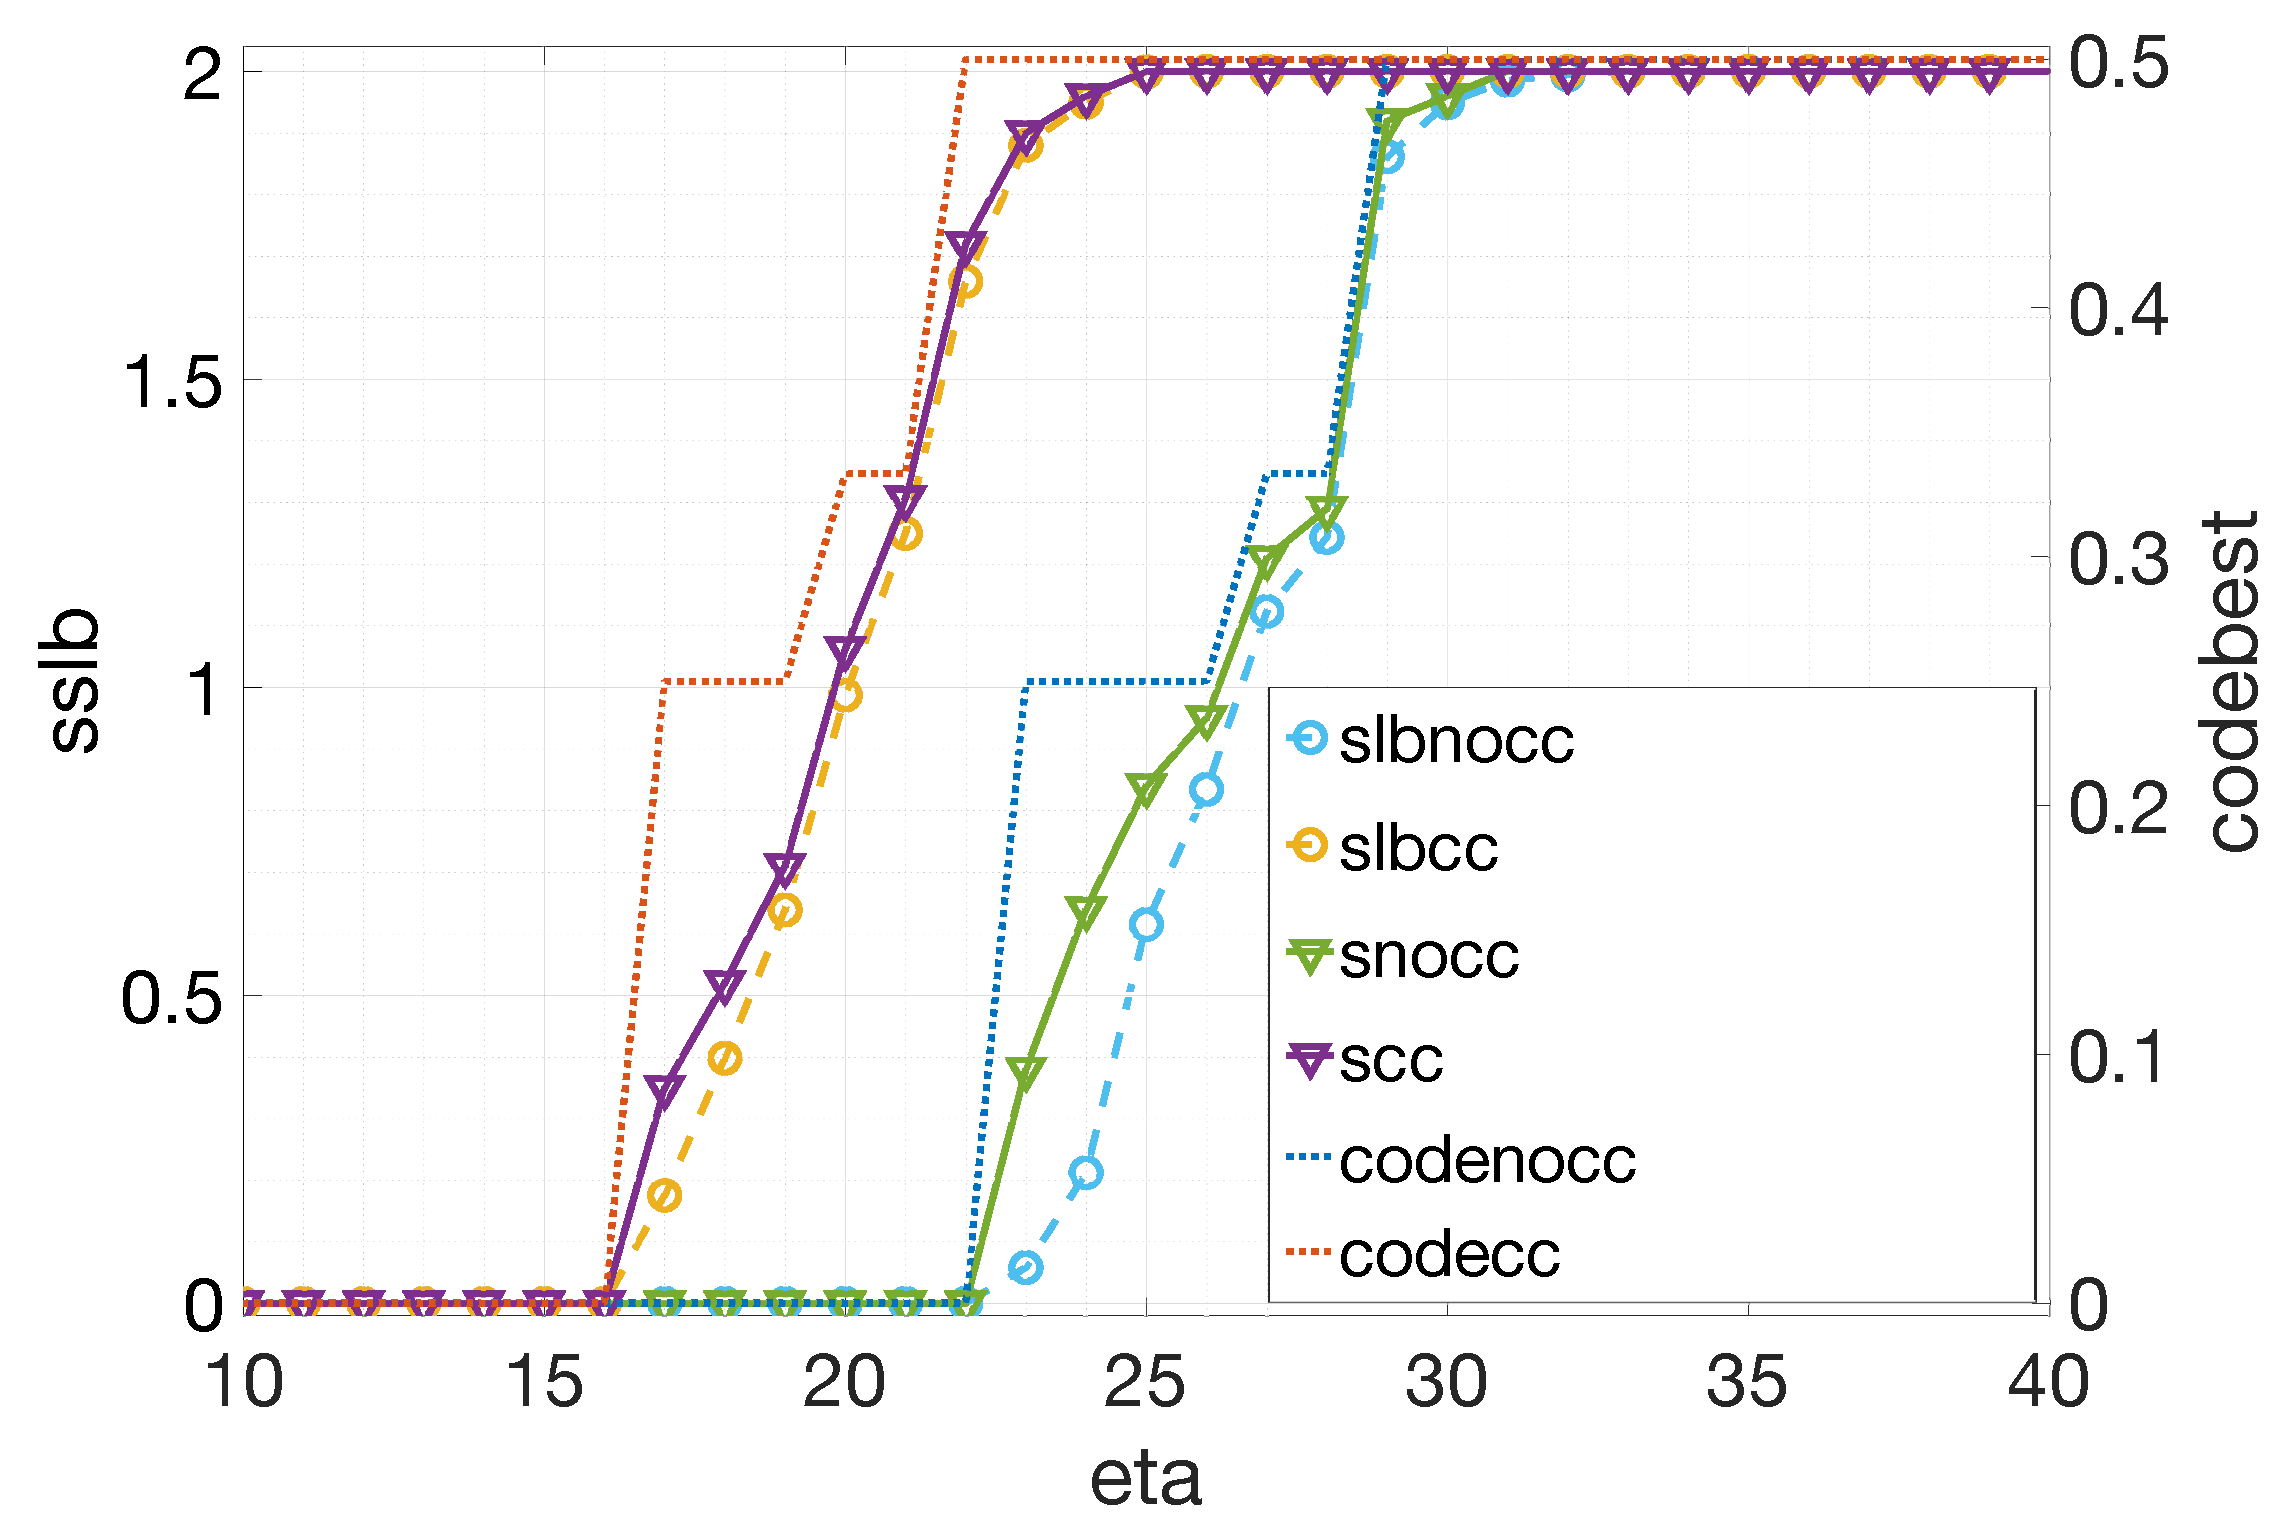
\includegraphics[width=\columnwidth]{Figures/sescompare_240111.eps}
    \caption{Comparison of SE $S$ (solid) and its lower bound 
             $\rbSLB$ (dotted) from CLO versus $\eta$ for $\rbJmax = 2$,
             $\rbMreq = \rbMtot/3$ and $\rbpreq = 0.1$ (left) and corresponding
             optimum rates $\rbRcopt$ (right).} 
    \label{fig:4}
\end{figure}

As the bit-rate constraint in {12} ensures for the chosen $\rbMtot$ 
that we have an average of 4 bits per subcarrier and the 
highest available $\rbRc$ is $\frac{1}{2}$, the maximum achievable SE is 2 
information bits per subcarrier. As seen in Fig.~\ref{fig:4}, $\rbSLB$ lower-bounds
$S$ with the bound tightening as we increase $\eta$. The 
steep changes in SE observed at $\eta \in \{17, 20, 22\}~\text{dB}$ for the 
case with CC and $\eta \in \{23, 27, 29\}~\text{dB}$ for the case without CC,
resp., result from changes in $\rbRcopt$. This change corresponds to 
the optimizer selecting a higher $\rbRcopt$ which maximizes $\rbSLB$. 
As the bit-rate constraint in {12} ensures for the chosen $\rbMtot$ 
that we have an average of 4 bits per subcarrier and the 
highest available $\rbRc$ is $\frac{1}{2}$, the maximum achievable SE is 2 
information bits per subcarrier. As seen in Fig.~\ref{fig:4}, $\rbSLB$ lower-bounds
$S$ with the bound tightening as we increase $\eta$. The 
steep changes in SE observed at $\eta \in \{17, 20, 22\}~\text{dB}$ for the 
case with CC and $\eta \in \{23, 27, 29\}~\text{dB}$ for the case without CC,
resp., result from changes in $\rbRcopt$. This change corresponds to 
the optimizer selecting a higher $\rbRcopt$ which maximizes $\rbSLB$. 
Clearly, in this case, using a CC improves the SE performance 
by approximately $6~\text{dB}$. Finally, in Fig.~\ref{fig:5}, we compare $\bar{J}$ with 
its upper bound $\bar{J}_{\text{UB}}$ from CLO.

\begin{figure}[htbp]
    \centering
\psfrag{nnub}[c][c]{\scriptsize $J,~\rbJUB~\rbJUBunit$} 
\psfrag{nubnocc}[c][c]{\scriptsize \hspace{4em}$\rbJUB~\rbJCLOnocc$} 
\psfrag{nubcc}[c][c]{\scriptsize \hspace{4em}$\rbJUB~\rbJCLOcc$}  
\psfrag{nnocc}[c][c]{\scriptsize \hspace{4em}$\bar{J}~\rbJSimnocc$} 
\psfrag{ncc}[c][c]{\scriptsize \hspace{4em}$\bar{J}~\rbJSimcc$}
    \psfrag{eta}[c][c]{\scriptsize $\rbEtaDB$}
    \psfrag{codenocc}[c][c]{\scriptsize \hspace{2em}$\rbRcopt$-no CC}
    \psfrag{codecc}[c][c]{\scriptsize \hspace{2em}$\rbRcopt$- CC}
    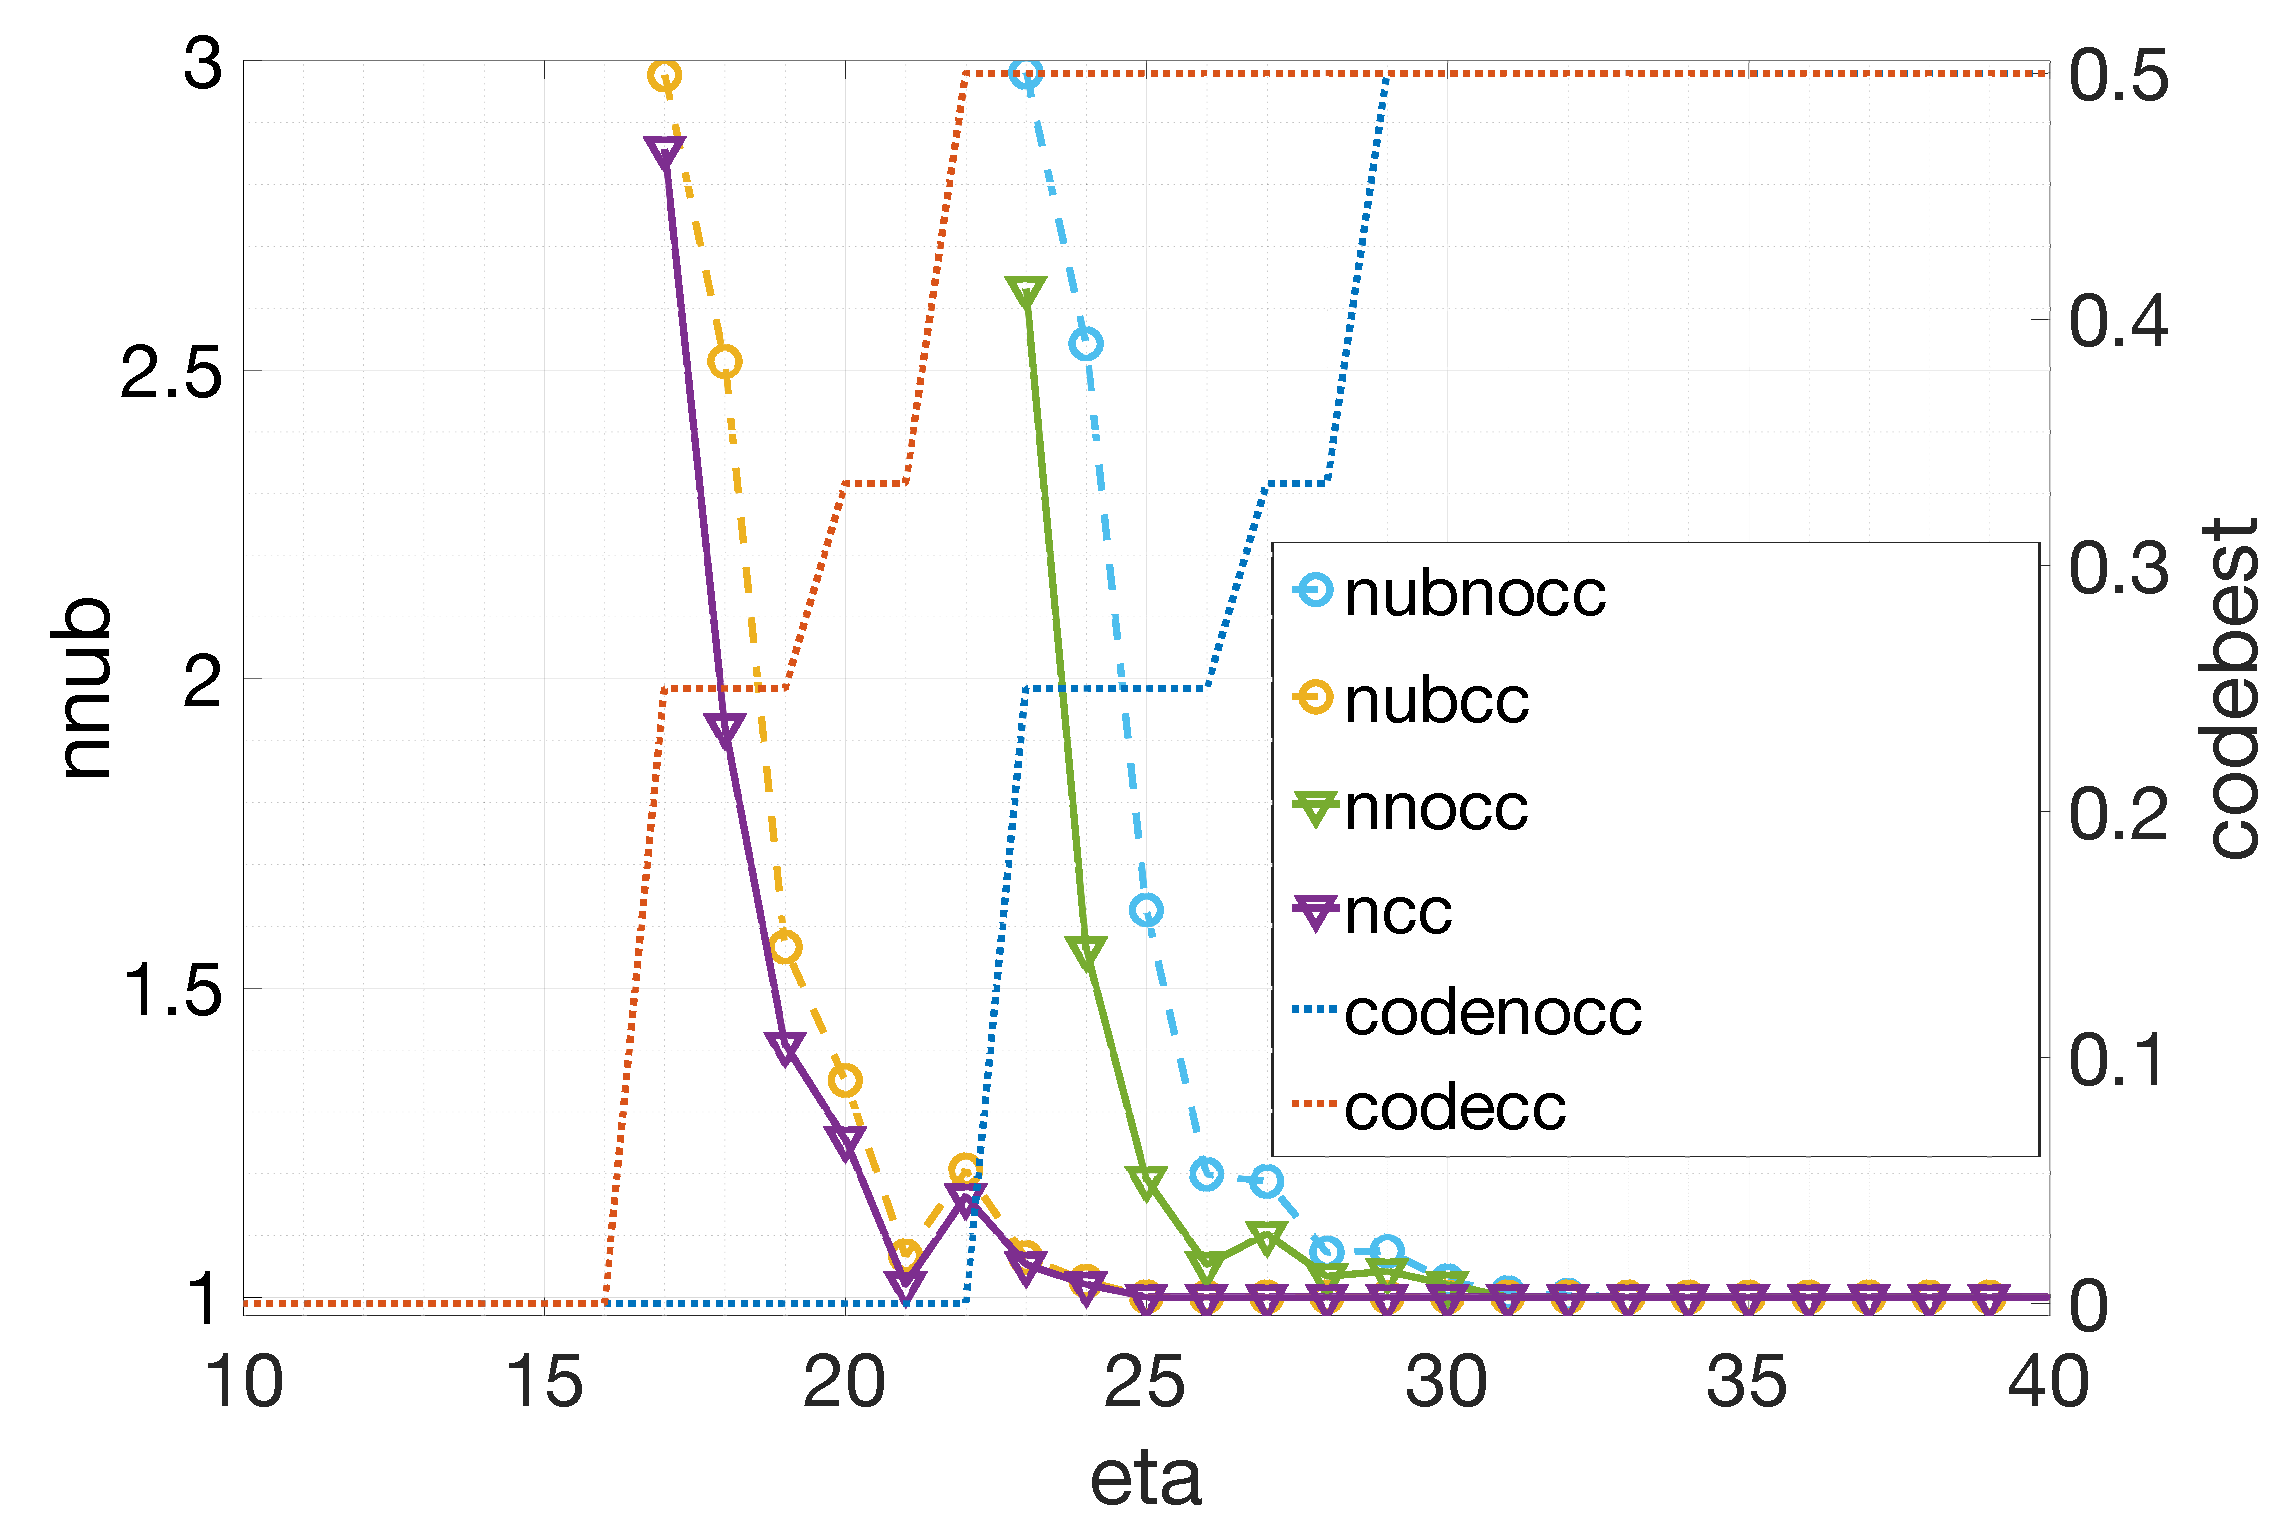
\includegraphics[width=\columnwidth]{Figures/nrscompare_240111.eps} 
    \caption{Comparison of average number $\bar{J}$ (solid) of transmissions
             per packet and its upper bound $\bar{J}_{\text{UB}}$ (dotted)
             from CLO versus $\eta$ for $\rbJmax = 2$, $\rbMreq = \rbMtot/3$
             and $\rbpreq = 0.1$ (left) and corresponding optimum rates
 $\rbRcopt$ (right).}
\label{fig:5}
\end{figure}
As expected, for a certain $\rbRcopt$, at low $\eta$, a large $\bar{J}$ is
observed, which decreases as $\eta$ increases while improving
$S$. The observed steep changes in $\bar{J}$ and $\bar{J}_{\text{UB}}$ correspond to changes of $\rbRcopt$ as discussed for $S$ in Fig.~\ref{fig:4}. Here, although
it leads to an increase in $D$, the optimizer may select an $\rbRcopt$
with higher $\bar{J}_{\text{UB}}$ as the goal is to maximize the $\rbSLB$.
\newpage
changes of $\rbRcopt$ as discussed for $S$ in Fig.~\ref{fig:4}. 
Here, although it leads to an increase in $D$, the optimizer may select 
a $\rbRcopt$ with higher $\bar{J}_{\mathrm{UB}}$ as the goal is to maximize 
$\rbSLB$.

\section{Conclusions}
\label{sec:5}
This paper proposes a \myCLO{} scheme to use \myLDPC{} coding together with \myCC{} protocols in a \myUCRS{} to maximize the \mySU{} \mySE{},assuming second-order channel state information is available at the \mySU{} transceiver. The \mySE{} is maximized subject to certain
interference and \myQoS{} constraints using an optimum \myJBPL{} and \myCA{} at the \mySU{} \myTX{}. A \myTHARQ{} type \myII{} is utilized in this system, which aims to improve \mySU{} transmission reliability by combining the signals from subsequent retransmissions using \myEGC{}. In particular, lower and upper bounds on the achievable \mySE{} are comparably tight over a large range of signal-to-noise ratios and the required number of transmissions, obtained over a \myTF{}-selective
fading channel using a constrained optimization approach. If the latter can be done in real time, it might serve as a basis for a more elaborated adaptation beyond the presented basic scheme.
While the current paper discusses a single \mySU{} and a single \myPU{} \myUCRS{} utilizing a \myTHARQ{} type \myII{} with \myCC{}, future research will focus on enhancing the \myTHARQ{} to type \myIII{} utilizing incremental redundancy along with testing the \myCLO{} scheme on a more complex \myUCRS{}.


\bibliographystyle{IEEEtran}
\bibliography{References}
\end{document}

